% ------------------------------------------------------------------------------
% AVR Synthesizer report
% Matt Bagnara
%
% Copyright: Creative Commons Attribution 4.0 International License
%            http://creativecommons.org/licenses/by/4.0
% Date: May 2014
% ------------------------------------------------------------------------------

% -------------------------------------------------------------------------------
% Preamble
% -------------------------------------------------------------------------------
\documentclass[bibtotocnumbered,abstract=on,paper=a4,fontsize=12pt,parskip=on,halfparskip=on]{scrartcl}		% KOMA article

\usepackage[a4paper,pdftex,margin=1in]{geometry}										% A4paper margins

\usepackage[english]{babel}
\usepackage[protrusion=true,expansion=true]{microtype}	
\usepackage{amsmath,amsfonts,amsthm,amssymb}
\usepackage{graphicx}
\usepackage[ocgcolorlinks]{hyperref} % for links in TOC
\usepackage{tabularx} % for better table spacing
\usepackage{appendix} % appendix in TOC
\usepackage{listings} % for software listings in appendix
\usepackage{xcolor}
\usepackage{float}
\usepackage{pgfgantt} % for gantt project schedules
% lscape.sty Produce landscape pages in a (mainly) portrait document.
\usepackage{lscape}
% ------------------------------------------------------------------------------
% Definitions (do not change this)
% ------------------------------------------------------------------------------
\AtBeginDocument{\setlength{\parfillskip}{1em plus 1fil}}% instead of 1em plus 1fil
\newcommand{\HRule}[1]{\rule{\linewidth}{#1}} 	% Horizontal rule
\makeatletter							% Title
\def\printtitle{%						
    {\centering \@title\par}}
\makeatother									

\makeatletter							% Author
\def\printauthor{%					
    {\centering \large \@author}}				
\makeatother							
\hypersetup{colorlinks=false,linkcolor=blue}
\setkomafont{disposition}{\normalfont \bfseries}
\lstset{language=c}          % Set your language (you can change the language for each code-block optionally)
\lstdefinestyle{makefile}
{
  numberblanklines=false,
  language=make,
  tabsize=4,
  frame=L,
  keywordstyle=\color{red},
  identifierstyle=,%plain for make,
  breaklines=true,
  basicstyle=\footnotesize\ttfamily,
}

\lstdefinestyle{plaintext}{
  belowcaptionskip=1\baselineskip,
  breaklines=true,
  xleftmargin=\parindent,
  showstringspaces=false,
  basicstyle=\footnotesize\ttfamily,
}
\lstdefinestyle{customc}{
  belowcaptionskip=1\baselineskip,
  breaklines=true,
  frame=L,
  xleftmargin=\parindent,
  language=C,
  showstringspaces=false,
  basicstyle=\footnotesize\ttfamily,
  keywordstyle=\bfseries\color{green!40!black},
  commentstyle=\itshape\color{purple!40!black},
  identifierstyle=\color{blue},
  stringstyle=\color{orange},
}
 \newcolumntype{L}{>{\raggedright\arraybackslash}X}

 % below colors for gannt
  \definecolor{barblue}{RGB}{153,204,254}
  \definecolor{groupblue}{RGB}{51,102,254}
  \definecolor{linkred}{RGB}{165,0,33}
  \setganttlinklabel{s-s}{START-TO-START}
  \setganttlinklabel{f-s}{FINISH-TO-START}
  \setganttlinklabel{f-f}{FINISH-TO-FINISH}

%---------------------------------------
% Higher number (default = 1000)        % reduces widows and orphans
\widowpenalty=9999
\clubpenalty=9999
%---------------------------------------

% ------------------------------------------------------------------------------
% Metadata (Change this)
% ------------------------------------------------------------------------------
\title{	\normalsize \textsc{Senior Design} 	% Subtitle of the document
		 	\\[2.0cm]													% 2cm spacing
			\HRule{0.5pt} \\										% Upper rule
			\LARGE \textbf{\uppercase{Cost-Efficient Analysis \& Generation of Polyphonic Music}}	% Title
			\HRule{2pt} \\ [0.5cm]								% Lower rule + 0.5cm spacing
			\normalsize \today									% Todays date
		}

\author{
		Matt Bagnara\\	
		Purdue University\\	
		ECET Department\\
    West Lafayette, Ind.\\
    \texttt{mbagnara@purdue.edu} \\ 
    \vskip 1cm 
    \scriptsize{AVR synthesizer $\cdot$ xmega $\cdot$ PS/2 $\cdot$ polyphonic music}\\
}


% ------------------------------------------------------------------------------
% Maketitle
% ------------------------------------------------------------------------------
\begin{document}
\begin{titlepage}
\thispagestyle{empty}				% Remove page numbering on this page

\printtitle									% Print the title data as defined above
  	\vfill
\printauthor								% Print the author data as defined above
    \vfill
    Signed: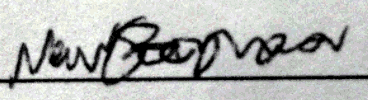
\includegraphics[height=1cm]{img/signature.png}\\
This report and project is submitted willingly as my own works. This document is licensed under a Creative  Commons Attribution-ShareAlike 4.0 International License.
\end{titlepage}
\newpage
% ------------------------------------------------------------------------------
% Begin document
% ------------------------------------------------------------------------------
\begin{abstract}
The problem of an easy-to-use music-making device has been one that countless designers have tackled with a different approach. The balance between niche usage, low cost, and usability has been difficult to balance. Many designs that exist are for specific usages and the typical unification of these devices may seem redundant. Also, the marriage between such a device and hobbyist development may be too focused. The objective of this project is to design and construct a polyphonic digital synthesizer. Unification of the device into an educational kit would satisfy the satisfy the curiosity of the hobbyist. A successful synthesizer will require a well-constructed input device and a microcontroller or processing platform. The synthesizer shall incorporate pulse, triangle, and noise tracks, as well as a means of mixing/synthesis. envelopes are anticipated, as they would allow much more musicality in dynamics. financially, the construction of the synthesizer is to remain within a set budget. optimally, the synth will be able to play music in real-time by the user and read data from a memory a modest key entry device shall be constructed for the user to interact with the hardware directly. the synthesizer should also include the ability to configure \& display the interaction to the user in some kind of gui. the intent of this project is to construct a synthesizer that could be used by hobbyist and beginners alike. this would require an interface with enough usability for both amateurs and hobbyists.

The process of creating a synthesizer of this nature requires looking at the problem from the viewpoint of the users who would be using it. The device was created using low-cost materials, but also looked advanced into emerging technologies such as the XMEGA architecture. The development was done in such a way to facilitate free and fair-use of all development tools, and facilitated the knowledge of skills that would be practical and useful.  This motivated the design of the software to all be accomplished using a POSIX environment. Also, the choice to use a PS/2 keyboard married legacy hardware, and new. The keyboard was chosen as an item that many users may have lying around could just plug-in without purchasing expensive hardware. This design caters to students and hobbyists alike.

The results of the design process display a functioning synthesizer prototype that is able to play real-time music, and also play recorded data. The project functions as a whole, only needing finalizations on the user-interface to conjoin the to modes of operation. Polishing is still needed, and the testing thus far reflects that. Nonetheless, this design is still a prototype with future capabilities down the pipeline.

\end{abstract}
\newpage
\begin{tableofcontents}
\end{tableofcontents}
\newpage
  \parskip1em

\section{Introduction}
  \subsection{Needs}
Electronic synthesizers are internationally found as means of communicating creative musical content. Chiptune is an an application of electronic synthesizers that emulate the classic 8-bit or early electronic music using the limited hardware of the time. While the ability to interpret sound data directly to a synthesizer is not new, the investigation of such a project would be an enjoyable learning experience, and perhaps create a new approach to an existing product.  The device could be directed towards construction as a kit; as such the intended users could be hobbyists and students who wish to construct a device they can use, while learning from it. This covers the major initial decision to license the project as it has been. The design and customization can be tailored to a specific usage. Also, the usage of limited hardware is anticipated to cost less.

A typical synthesizer is capable of real-time synthesis \& playback. Songs are likely stored in a removable media which can be swapped for recording. The sound emitted from a typical polyphonic electronic synthesizer is in the form of arbitrary waveforms, including a noise track for percussion.

Synthesizer kits are also available to be built and operate. The user may prefer to purchase a commercial available option, However, a custom-made synthesizer will offer all the ability of hardware chiptune creation with the functions of a modern synthesizer at a modest price preferable under USD\$200. 
  \subsection{Objectives}
The objective of this project is to design and construct a polyphonic digital synthesizer. A Successful synthesizer will require a well-constructed input device and a microcontroller or processing platform. The synthesizer shall incorporate pulse, triangle, and noise tracks, as well as a means of mixing/synthesis. Envelopes are anticipated, as they would allow much more musicality in dynamics. Financially, the construction of the synthesizer is to remain within a set budget. Optimally, the synth will be able to play music in real-time by the user and read data from a memory A modest key entry device shall be constructed for the user to interact with the hardware directly. The synthesizer should also include the ability to configure \& display the interaction to the user in some kind of GUI. The intent of this project is to construct a synthesizer that could be used by hobbyist and beginners alike. This would require an interface with enough usability for both amateurs and hobbyists.
\clearpage
\section{System Overview}
The main idea is to create a synthesizer that can interface the user through a keyboard or other key entry device. The input shall allow the instrument to be played in real-time. The user interface or display can be navigated to select different sounds or waveforms(instruments/voices) in this mode. The secondary mode allows the playback of external music data which can be connected to a workstation computer to play data. The user display would be utilized in this mode to select the music data or file to be played. The output audio would be a consumer audio interface which can be later amplified or connected to a speaker.

  \subsection{System Requirements}
    \subsubsection{Marketing Requirements}
      \begin{enumerate}
        \item The cost shall stay within a low level budget in a non-niche market.
        \item The synthesizer shall contain an intuitive interface for amateurs and hobbyists.
        \item The synthesizer should provide playback of recorded digital data.
        \item The synthesizer should provide real-time playtime of data.
        \item The synthesizer should synthesize digital data as polyphonic music.
      \end{enumerate}
    \subsubsection{Requirement Specification}
    \begin{table}[H]
      \caption{Requirements}
      \vskip 0.3cm
      \begin{tabularx}{\linewidth}{ p{2.0cm} X X }
        \textbf{Marketing Requirement} & \textbf{Engineering Requirement} & \textbf{Justification} \\
          \hline
        1. & The budget for the synthesizer will be USD\$200, but the total cost shall not exceed USD\$225. & The budget constraint will provide a modest price.\\
          \hline
        2. & The synthesizer shall offer a visual user interface in the form of a two-line character LCD with a lit screen. & To provide an easy, intuitive, powerful control interface.\\
          \hline
        2. & The synthesizer will not contain more than three sublevels of menus. & Simple, easy to use interfaces that are organized will be logical to follow.\\
          \hline
        3. & The synthesizer will provide interpretation of a digital format for playback. Dat speed from from storage should be at least 8 Mbit per Second. & Playback of recorded data will require an abstraction of  music into a data representation.\\
          \hline
        4. & The synthesizer will offer a method for external storage following an SD (Secure Digital) SPI interface. & External storage may easily be interfaced by a PC system for generating digital data for playback.\\
          \hline
        5. & The synthesizer will offer interface that will facilitate playing as an instrument with a response time less than 5ms. & Realtime playback will require a method the user can play the instrument.\\
          \hline
        6. & The total output frequency response should be between 30 and 12KHz. & Audio playback shall play within the average response of the human ear.\\
          \hline
        7. & The synthesizer will generate no less than three voices, including one distinct square, sine, and noise voice to be played simultaneously. & Music composed of individual waveforms can be mixed to represent a wide variety of polyphonic music.\\
      \end{tabularx}
      \end{table}
  \subsection{Concept Generation \& Evaluation}  
    \subsubsection{Concept Generation Tree}
    \begin{figure}[H]
      \centering
      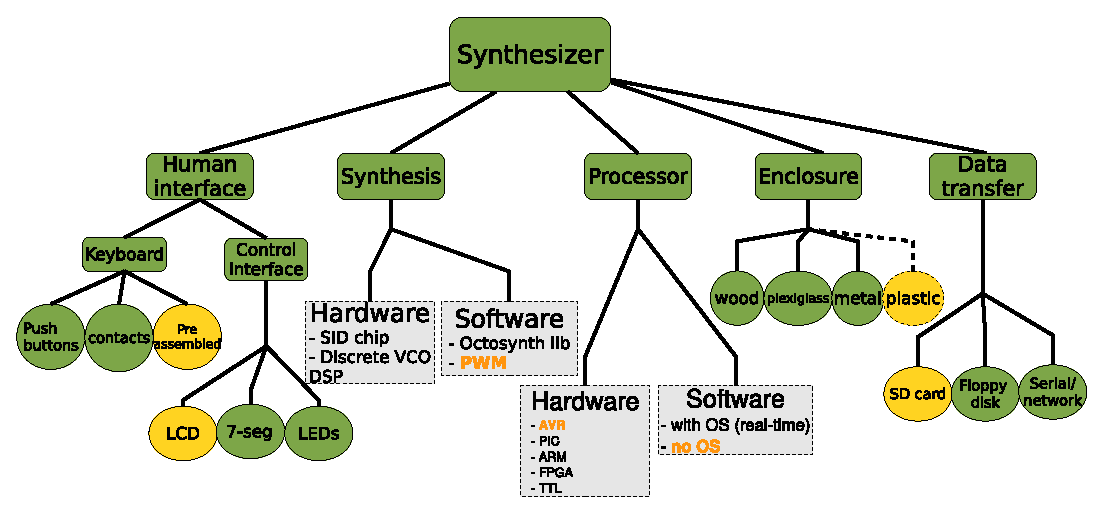
\includegraphics[width=\linewidth]{img/fig_concepttree}
        \caption{Concept Generation Tree displaying selected items in Orange}
    \end{figure}
    \subsubsection{Concept Blocks}
    \begin{enumerate}
        \item{Main Processor}
          The main processor will handle user input from the keyboard and the user interface. It will drive the user display, and handle the data-transfer abstraction from the user. It will also interpret the music data, whether it be MIDI, etc., and generate data for use in synthesis.
        \item{Keyboard}
          The keyboard provides the basic user interaction for real-time music creation. The keyboard may be a prefabricated accessory, or may become its own block.
        \item{User Interface}
          The user interface allows the user to select which song to play on the external media.
        \item{Synthesis}
          The synthesis software block is where the waveform generation occurs. Music data generated by the processor is formed into arbitrary waveforms and amplified using an envelope function\
        \item{Enclosure}
          The enclosure will provide adequate housing for its use as a synthesizer. Looks and aesthetics will cater to usability for amateurs and hobbyists and could feature a retro design.
        \item{Data Transfer}
          The data-transfer will provide support for external media. This will facilitate the transfer of external music data for use in playback. The data can be fabricated on a workstation computer and played back on the synthesizer through this transfer interface.
      \end{enumerate}


  \subsection{System Decomposition}
      \begin{table}[H]
      \caption{Synthesizer Subsystem}
      \vskip 0.3cm
      \begin{tabularx}{\linewidth}{  l X }
        \textit{Module} & Synthesizer \\
        \hline
        \textit{Inputs} & External DC power: 5V dc\\
          & External Media for data storage playback: SD card\\
        \hline
        \textit{Outputs} & Polyphonic music playback through consumer audio specification. TRS connector\\
        \hline
        \textit{Functionality} & Provide polyphonic synthesis of keyed music by the user and playback of recorded media\\
      \end{tabularx}
      \end{table}
      %====
      \begin{table}[H]
      \captionof{table}{Processor Platform Subsystem}
      \vskip 0.3cm 
      \begin{tabularx}{\linewidth}{  l X }
        \textit{Module} & Processor Platform \\
        \hline
        \textit{Inputs} & Serial or MIDI interface from key: PS/2\\
          & data interface to tertiary storage: SPI SD card\\
          & Logic signal from keyboard: 5V dc\\
          & Power: 3.3V dc\\
        \hline
        \textit{Outputs} & Logic signal for LCD display:3.3V dc parallel(8-bit)\\
          & Digital buffers to synthesis block: 3 voices, 256 bits\\
        \hline
        \textit{Functionality} & To drive user interface of the synthesizer and manage data acquisition into the synthesis of polyphonic PWM waveforms.\\
        \hline
        \textit{Rationale} & Provide method for interchangeable Processor interface for future expandability.\\
      \end{tabularx}
      \end{table}
      %====
      \begin{table}[H]
      \caption{SD Card Subsystem}
      \vskip 0.3cm 
      \begin{tabularx}{\linewidth}{  l X }
        \textit{Module} & SD Card\\
        \hline
        \textit{Inputs} & \\
           & Power:5V dc\\
           & PS/2: psuedo I2C interface\\
        \hline
        \textit{Outputs} & PS/2: psuedo I2c interface \\
        \hline
        \textit{Functionality} & \\
        \hline
        \textit{Rationale} & \\ 
      \end{tabularx}
      \end{table}
      %====
      \begin{table}[H]
      \caption{PS/2 Keyboard Subsystem}
      \vskip 0.3cm 
      \begin{tabularx}{\linewidth}{  l X }
        \textit{Module} & PS/2 Keyboard \\
        \hline
        \textit{Inputs} & Human interface through individual keys\\
           & Power:5V dc\\
           & PS/2: psuedo I2C interface\\
        \hline
        \textit{Outputs} & PS/2: psuedo I2c interface \\
        \hline
        \textit{Functionality} & Provide synthesis of output digital logic voltages for music playback.\\
        \hline
        \textit{Rationale} & Provide method for interchangeable user-input.\\
      \end{tabularx}
      \end{table}
      %====

      \begin{table}[H]
      \caption{Synthesis Subsystem}
      \vskip 0.3cm 
      \begin{tabularx}{\linewidth}{  l X }
        \textit{Module} & Synthesis\\
        \hline
        \textit{Inputs} & Digital buffers to synthesis: 3 voices, 256 bits.\\
           & 5V dc\\
        \hline
        \textit{Outputs} & Audio signal for consumer electronics: 0.894Vpp\\
        \hline
        \textit{Functionality} & Provide synthesis of output digital logic voltages and mixing for music playback.\\
        \hline
        \textit{Rationale} & Choosing to create a discrete voltage controlled oscillator would allow a customized solution. It would allow multiple voices to generate their own waveforms in parallel, creating a form of modularity. It could be easily controlled using digital potentiometers.  Mixing could easily be done at the end. The usage of envelopes would be facilitated through use of VCA (voltage controlled amplifiers)\\
      \end{tabularx}
      \end{table}
      %====
      \begin{table}[H]
      \caption{LCD Subsystem}
      \vskip 0.3cm
      \begin{tabularx}{\linewidth}{  l X }
        \textit{Module} & User interface(LCD) \\
        \hline
        \textit{Inputs} & Power: 5V dc\\
           & Logic from processor: 3.3V dc parallel 8 bits\\
        \hline
        \textit{Outputs} & Human interface\\
        \hline
        \textit{Functionality} & Provides the user with an interface for navigation of features.\\
        \hline
        \textit{Rationale} & An LCD would allow the creation of a useful interface. Can create intuitive interfaces through use of graphical menus and display of information.\\
      \end{tabularx}
      \end{table}

      \begin{center}
      \vskip 1cm
        \centering
          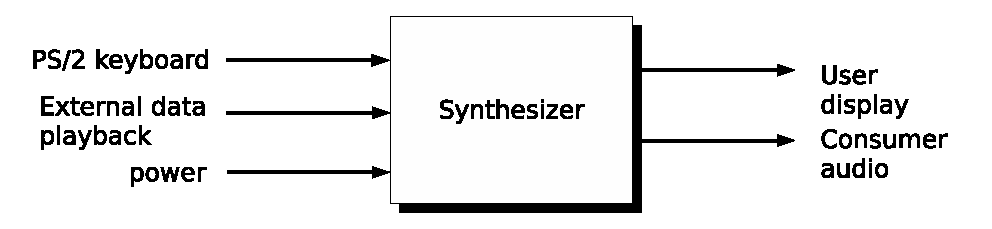
\includegraphics[width=\linewidth]{img/fig_level0}
          \captionof{figure}{Level 0 - Synthesizer}
      \vskip 1cm
        \centering
          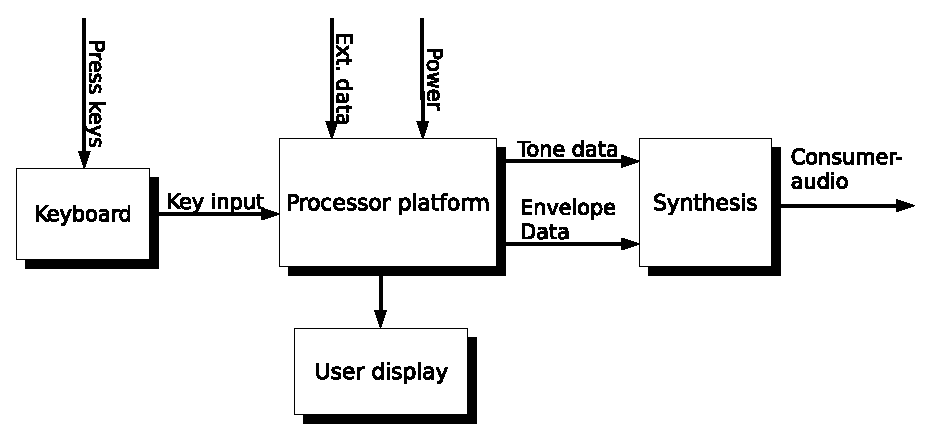
\includegraphics[width=\linewidth]{img/fig_level1}
          \captionof{figure}{Level 1 - Synthesizer}
      \vskip 1cm
      \end{center}
  \subsection{Developmental Plan}
    The development plan for the synthesizer will divide between the hardware components and the software development. About 25\% of the project will involve hardware. The following table will record this breakdown of the subsystems.\\
    \begin{table}[H]
    \caption{Itemized subsystem development}
    \vskip 0.3cm
    \small
    \begin{tabularx}{\linewidth}{  l p{2.1cm} l X X }
      \textbf{Subsystem} & \textbf{Dev Ratio} & \textbf{Dependencies} & \textbf{Software} & \textbf{Hardware}\\
      \hline
      PS/2 keyboard & 0.10 & Processor & PS/2 driver & Connector:proto\\
      LCD display & 0.10 & Processor & LCD driver & protoboard\\
      External SD & 0.20 & Processor & SD library available & \\
      Synthesis & 0.25 & Processor & Software synthesis & Hardware mixer\\
      Processor & 0.45 & N-A & Software operating system & Dev board\\
    \end{tabularx}
    \end{table}

    The development ratio gives an idea of what amount of time will be spent on each subsystem. 

    The order in which development shall carry out will tentatively follow this pattern:
    \begin{enumerate}
      \item{\textbf{Processor}}\hfill \\
      Processor development shall start first and begin with the hardware board being created or chosen. Currently, the choices are to use an AVR developmental board or an AVR programmer using a custom created proto-board or perf-board. 

      The software component will also begin and initial development can begin concurrently until the build environment is established. Current software choices are leaning toward the usage of a Real Time Operating System (RTOS) The processor software will be a large component of this development as the abstractions for runtime are formed in this stage.
      \item{\textbf{Synthesis}}\hfill \\
      Synthesis development will be tightly integrated with the processor platform. The software development can begin first, following usage of the processor as its resource. The wavetable and sampling routines are to be developed at this point. Following creation of the software synthesis component, the hardware DAC may be chosen for sound output.
      \item{\textbf{External SD}}\hfill \\
      Perhaps one of the more complex peripherals, the SD storage device shall be incorporated into the runtime of the processor. The current anticipated solution is to include an SPI\cite{FFoust2004} SD library and work with that. The hardware component of the SD interface shall be incorporated into the development board being used.
      \item{\textbf{PS/2 Keyboard}}\hfill \\
      The PS/2 keyboard requires no assembly because it shall be obtained as a finished component. The software-level driver shall be written into the runtime of the processor, and will be interfaced via serial peripheral on the processor platform\cite{website:avinash}. The hardware port will be placed on the development board for testing and usage.
      \item{\textbf{LCD Display}}\hfill \\
      The LCD display requires no assembly because it shall be obtained as a finished component. The software-level driver shall be written into the runtime of the processor, and will be interfaced via the software specification of the LCD display, most likely being SPI. The hardware port will be placed on the development board for testing and usage.
      \item{\textbf{Mechanical Plan}}\hfill \\

      Mechanical chassis focuses on a small profile enclosure. The material of choice for the enclosure will most likely be wood or 3D printed to keep costs low. Figures \ref{fig:3d1} \&  \ref{fig:3d2} display a rendering using \textit{Valve Hammer Editor} of what the chassis may look like. It features a mounting for the LCD display and main power switch on the front. The rear will provide fixtures for the DB-9, power, and TRS connectors. The right side will feature a slit to clear the turn potentiometer as it protrudes from the enclosure.
    \end{enumerate}

      \clearpage
\section{Subsystem Technical Descriptions}
  Much of the testing being done will feature the debug menu which will be incorporated into the development board. The debug menu will feature self-tests documented in \nameref{sec:testing-documentation} to use to verify functionality of the peripherals. The tests will run using an external serial interface on the processor and can be accessed using a serial terminal.\par
  \subsection{Synthesis subsystem}
    The Synthesis subsystem consists of the software \& hardware which creates the output waveform from the digital data being created by the processor. This subsystem is composed of software routines that create a audio buffer to write out to the DAC as well as the routines for mixing the separate buffers. This subsystem is vital to the tonal generation of music. First of all, to verify the proper operation of the synthesis portion, the waveshape, frequencies, mixing, and other parameters need to be validated. 

    Synthesis is being done in both hardware and software, so both components are required. To ensure proper generation of arbitrary waveforms, the output of the synthesizer shall be connected to a 50 ohm terminated oscilloscope. The visual oscilloscope tube can be used to capture the correct waveshape for each voice. Next, the frequency range of the synthesizer will be tested using the built-in sweep function in the debug menu. The oscilloscope can, again, be used to capture the frequency vs. time data to verify this part. The voltage levels of the waveforms can also be checked at this point. The final task to verify would be the mixing capability of the synthesizer by generating polyphonic tones in the form of two, and three note chords. This may be verified by viewing a frequency-domain plot on the oscilloscope.
  \subsection{LCD display subsystem}
    The LCD unit consists of the LCD display, as well as the display driver being written on the software. The LCD subsystem will act as the user's interface to the synthesizer when it is being run in real-time for playback or for playback of premade audio. The purpose of this display is to provide the user with an interface. 

    The LCD will operate using a user-created driver and the output shall be connected using a parallel interface. First, the verification of the display of characters will simply be done by cycling through printable ASCII characters. This will be done using the functionality of the debug menu. Also, the processing of control characters and clearing the screen will be demonstrated using this same debug screen.
  \subsection{PS/2 Keyboard subsystem}
    The keyboard unit consists of the PS/2 display, as well as the PS/2 driver running in software. This subsystem is used to provide key entry to the synthesizer block. It is vital to the synthesizer as it provides the only keyed input from the user. It will be used as the musical keyboard, as well as the controls to the user-interface on the LCD. 
  \subsection{Processor subsystem}
    The processor platform subsystem consists of the microprocessor platform being used, as well as the software layer being run on it. This subsystem is the heart of the synthesizer platform, as it interfaces with all peripherals, and all software will be written on. 
    \vskip 0.25cm
    \textbf{Hardware}\hfill \\
    The hardware platform for this processor subsystem will be an ATXMega256D3. This processor will feature 256 kilobytes of programmable flash memory, and port-assignable timers. The selected clock will be a 16KHz crystal. Programming will be done via PDI using an AVRISP MKII. PWM timers output from the microcontroller mixed and filtered will be used to perform the waveform generation.
    \vskip 0.25cm
    \textbf{Software}\hfill \\
    The software of the processor platform will ideally provide hard or soft real-time support through use of a real-time operating system. The motivation of the operating system is to accomplish real-time tasks within stringent deadlines. \cite{0595375979}Because this system will be processing audio samples, a real-time operating system will be used to timely produce the music. As depicted in Figure ~\ref{fig:software0}, the software for the synthesizer will be divided into tasks which interface with a particular peripheral.
  \subsection{SD card subsystem}

   The SD unit consists of the SD card interface, as well as the software filesystem driver being used to interface via SPI. The SD subsystem provides the synthesizer a method to playback non-volatile memory or per-recorded sequences. To verify the proper functionality of the SD device, the creation of file handles, and reading of blocks should be demonstrated.

    The SD will operate using an available FAT\_FS \cite{website:fatfsnotes} library, and the input shall be connected using an SPI  interface. Because the synthesizer will only be reading music data, the demonstration will require the ability to read off the SD card. This subsystem is integrated into the processor platform, therefore, it requires the processor subsystem to be tested. The demonstration will require the creation of a file handle, and reading the blocks of data into memory of the processor. The debug program on the processor will read ASCII data off the SD card and output it via its external serial interface.\\

    \begin{figure}[h!]
      \centering
        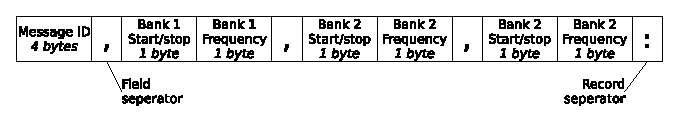
\includegraphics[]{img/fig_asciimessage}
        \caption{ASCII message structure}
        \label{fig_asciimessage}
    \end{figure}

    Figure~\ref{fig_asciimessage} above depicts the preliminary data-layout chosen for the scope of each playback sequence. This data represents a sequence of messages that composes a tune being read from the SD in ASCII mode. As a result, filesizes will be much larger, but this is at the expense of creating an easily modifiable human-readable format. 

    Next, the ASCII messages are then evaluated and an associating \texttt{order} object is created to represent the item. A library was designed for the purpose of representing a linked-list datastructure. An executive decision was made at this point to represent the data using a linked-list. Although a linked-list does not allow random-access of data, they provide insertions and deletions to occur in constant time $ \Theta(1) $\cite{sedgewick2011algorithms}. This was evaluated due to the amount of messages that would be processed. The library used consists of the \texttt{onode} structure which points to the data containing the actual music.

    \begin{figure}[h!]
      \centering
        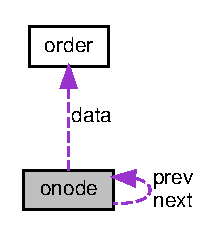
\includegraphics[]{img/structonode_coll_graph.eps}
        \caption{Collaboration Diagram for onode}
        \label{fig_onode}
    \end{figure}

      \begin{table}[H]
      \label{table_order}
      \small
      \centering
      \caption{Struct \texttt{order} Data Fields}
      \begin{tabularx}{0.4\textwidth}{ p{1.5cm} X }
        \hline
        int & id \\
        char & bank1\_startstop \\
        char & bank1\_note \\
        char & bank2\_startstop \\
        char & bank2\_note \\
        char & bank3\_startstop \\
        char & bank3\_note \\
        \hline
      \end{tabularx}
      \end{table}

    Figure \ref{fig_onode} shown above is used as the encapsulation method for the \texttt{order} tone data. The data is represented above in \ref{table_order} and this data is passed on to the synthesis block to process the indivudual messages that come in. Because these messages are passed asynchronously, they are not long-lasting in the life of the execution cycle. Transformation occurs fast, yet the structure used would allow future expandability for more complex tone messages.

\section{Testing Methods, Results and Evaluation}
  \subsection{Subsystem Test Plans}

      Testing for LCD unit functionality was successful as shown in Table~\ref{tab:lcd_unittest}. The testing was done on a stub development board ATMEGA16. Functionalities demonstrated were the ability to display two-line character buffers to the screen, presenting custom glyphs as characters, contrast adjust, and clearing the screen. The requirement for this test maps to requirement \#2 to provide an intuitive user interface. The LCD testing results will demonstrate this ability in conjunction with the keyboard to develop a menu system. See Appendix~\nameref{sec:testing-documentation} for test setup.

      Testing for the PS/2 was successful using the ATMEGA16 as shown in Table \ref{tab:ps2_unittest}. Functionalities demonstrated were the ability to read scancodes from the keyboard on key press and key release events. Because the intent is to use the alphanumeric keyboard for key entry, only level1 scancodes will need to be interpreted. This test maps to the requirement to provide an intuitive user interface, as well as a means to input data for playback. See Appendix~\nameref{sec:testing-documentation} for test setup.


      Testing for the SD storage was successful as shown in Table \ref{tab:sd_unittest}. The SD was damaged during testing and yielded inconclusive evidence. With recent acquisition of the SD card breakout board, testing can continue. The requirement for this test will map to requirement \#3, and \#4. Although inconclusive at this point, the testing will continue. See Appendix~\nameref{sec:testing-documentation} for test setup.


Testing of the synthesis unit is complete in conjunction with the processor platform testing as depicted in Table \ref{tab:synthesis_unittest}. Because of the tight integration between these two subsystems, development was done on the same platform. Functionality to demonstrate is the ability to generate compound waveforms from arbitrary waveform buffers. The simplest of these would be to output an arbitrary waveform scaled to frequency f. This will be used to generate a chromatic frequency sweep. Noise, generation will follow. Superfixing two waveforms will create two simultaneous tones at 440Hz and 460Hz. Three tones will be superfixed next to create deeper chord structure at 440, 460, and 520Hz. Finally, square and triangle waveforms are tested. This testing sequence will demonstrate the requirement of \#7 and \#6. See Appendix~\nameref{sec:testing-documentation} for test setup.


Testing of a processor platform demonstrates overall functionality of the microprocessor. Testing was be done in a stateless mode of operation to ensure proper functionality of the unit. Metrics observed in Table \ref{tab:processor_unittest} were poweron functionality, and PDI advertisement.

  \subsection{Integration Plans}

Integration of the subsystem blocks will follow an order which allows the system to be joined logically. The listing below illustrates the 5 phases of integration.

  \begin{enumerate}
    \item{Processor platform}
    \item{LCD display}
    \item{SD storage}
    \item{Synthesis}
    \item{PS/2 keyboard}
  \end{enumerate}

With the synthesizer, the initial block will be the processor platform. This will represent the base for which all subsequent tests will be dependent on. This subsystem is vital to all subsequent tests. 

Second, the LCD display will be added with its hardware and software functionality. This integration will be vital to provide the user with an interface that can be used for testing further on. The initial LCD test will be the same test used in the LCD subsystem testing because it is essentially the same.

Third, the SD storage will be integrated with its FAT library component, as well as the hardware interface. The testing for this stage will include reading ASCII data from the card and writing it to the LCD display. This test will be part of the debug system as it is being built for integration.

Next, the synthesis subsystem can be integrated with its software components. The synthesis subsystem will make usage of the incrementing debug system being built up. The tests of this integration will involve simple waveform generation, more sophisticated chord synthesis and generation, and noise track synthesis.

Last, the PS/2 keyboard will be integrated into the system. The PS/2 keyboard testing can be used in conjunction with the LCD to display an intuitive menu that can be navigated using the keyboard. Testing for this integration will facilitate the creation of a whole debug-menu system that can be navigated and displayed on the LCD.
The final system integration step will test some of the Engineering requirements as a whole to ensure proper functionality throughout. These tests will address the requirements listed in Table 2.1.2 . This will include tests of reading data from the SD card and playing back. Also, the system will need to allow real-time playback when set to that state.
  \subsection{Integration Testing}
      \begin{table}[H]
      \caption{Processor integration test}
      \footnotesize
      \vskip 0.3cm
      \begin{tabularx}{\linewidth}{ |p{2.1cm}|X|X|p{0.7cm}|p{0.6cm}|X| }
        \hline
        \multicolumn{2}{|l|}{\textbf{Test Writer}} & \multicolumn{4}{c|}{Matt Bagnara} \\
        \hline
        \multicolumn{2}{|l|}{\textbf{Test Case Name}} & {Integ-processor} & \multicolumn{2}{c|}{\textbf{Type}} & integration \\
        \hline
        \textbf{Description} & \multicolumn{2}{|>{\centering\setlength\hsize{2\hsize} }X|}{Includes the introduction of processor platform onto the testing board} & \multicolumn{2}{c|}{\textbf{Date}} & 11/22/13 \\
        \hline
        \textbf{Setup} & \multicolumn{2}{|>{\centering\setlength\hsize{2\hsize} }X|}{Connect processor power and setup as in Appendix J} & \multicolumn{2}{c|}{\textbf{Time}} & \\
        \hline
        \multicolumn{6}{|l|}{\textbf{Test}} \\
        \hline
        \textbf{Name} & \textbf{Action} & \textbf{Expected output} & \textbf{Pass} & \multicolumn{2}{X|}{\textbf{Comments}} \\
        \hline
        Poweron test & Connect +5V, +3.3V, GND on CONN6  & LED on board should light green & \checkmark & \multicolumn{2}{X|}{} \\
        \hline
        processor presence & See \nameref{processortest} & Should respond with device signature \texttt{0x1e9844} & \checkmark & \multicolumn{2}{X|}{} \\
        \hline
      \end{tabularx}
      \end{table}

Testing for the processor integration stage went successful. The stage of testing began with the testing board layout. The testing board layout is explained in Appendix J - Test Board. The processor is the first stage to be integrated onto the testing unit. This was done by simply inserting the processor assembly into the testing board via DIS1 and connecting the programmer to CONN1. The processor integration provides the base for which all subsequent integration steps will follow. For this reason, the processor integration needed to be checked for integrity while interfacing the testing board. The demonstrations for this integration step simply required power to be supplied correctly to the processor assembly, as well as detecting the presence of the processor by the PDI interface.

      \begin{table}[H]
      \caption{LCD integration test}
      \vskip 0.3cm
      \footnotesize
      \begin{tabularx}{\linewidth}{ |p{2.1cm}|X|X|p{0.7cm}|p{0.6cm}|X| }
        \hline
        \multicolumn{2}{|l|}{\textbf{Test Writer}} & \multicolumn{4}{c|}{Matt Bagnara} \\
        \hline
        \multicolumn{2}{|l|}{\textbf{Test Case Name}} & {Integ-LCD} & \multicolumn{2}{c|}{\textbf{Type}} & integration \\
        \hline
        \textbf{Description} & \multicolumn{2}{|>{\centering\setlength\hsize{2\hsize} }X|}{Includes the introduction of the LCD display library into the codebase along with connection} & \multicolumn{2}{c|}{\textbf{Date}} & 11/23/13 \\
        \hline
        \textbf{Setup} & \multicolumn{2}{|>{\centering\setlength\hsize{2\hsize} }X|}{Connect processor power and setup as in Appendix J} & \multicolumn{2}{c|}{\textbf{Time}} & \\
        \hline
        \multicolumn{6}{|l|}{\textbf{Test}} \\
        \hline
        \textbf{Name} & \textbf{Action} & \textbf{Expected output} & \textbf{Pass} & \multicolumn{2}{X|}{\textbf{Comments}} \\
        \hline
        Poweron test & Power board as before and plug LCD ribbon to CONN2 & LCD should light with a blue glow & \checkmark & \multicolumn{2}{l|}{$\displaystyle VSS= 4.96V, VCC= 3.28V$} \\
        \hline
        Contrast adjust & Adjust the potentiometer near CONN2 & Contrast should adjust for visibility per lighting condition & \checkmark & \multicolumn{2}{l|}{full range visible} \\
        \hline
        Display of text & Execute displayText routine \texttt{main.hex} & \texttt{Test text} should display on LCD display & \checkmark & \multicolumn{2}{X|}{} \\
        \hline
      \end{tabularx}
      \end{table}

Second stage of integration includes the physical LCD display along with software used by the LCD to interface. The reason for choosing the LCD to integrate second was to facilitate a means of standard output to be used for further integration tests. The LCD needs to be tested using its software library to ensure proper display and visibility of data. The first line of testing is to ensure proper voltage to the logic supply of the LCD as well as to the lighting unit of the LCD. Next, the contrast adjusting functionality is tested being integrated to the testing board to ensure proper visibility adjustment of the display. The library is put to the test being integrated into the development environment of the processor. Testing display of buffered text to the LCD was successful at this stage.

      \begin{table}[H]
      \caption{SD card integration test}
      \vskip 0.3cm
      \footnotesize
      \begin{tabularx}{\linewidth}{ |p{2.1cm}|X|X|p{0.7cm}|p{0.6cm}|X| }
        \hline
        \multicolumn{2}{|l|}{\textbf{Test Writer}} & \multicolumn{4}{c|}{Matt Bagnara} \\
        \hline
        \multicolumn{2}{|l|}{\textbf{Test Case Name}} & {Integ-SD} & \multicolumn{2}{c|}{\textbf{Type}} & integration \\
        \hline
        \textbf{Description} & \multicolumn{2}{|>{\centering\setlength\hsize{2\hsize} }X|}{Includes the introduction of the SD card library into the codebase along with connection} & \multicolumn{2}{c|}{\textbf{Date}} & 11/23/13 \\
        \hline
        \textbf{Setup} & \multicolumn{2}{|>{\centering\setlength\hsize{2\hsize} }X|}{Connect processor power and setup as in Appendix J} & \multicolumn{2}{c|}{\textbf{Time}} & \\
        \hline
        \multicolumn{6}{|l|}{\textbf{Test}} \\
        \hline
        \textbf{Name} & \textbf{Action} & \textbf{Expected output} & \textbf{Pass} & \multicolumn{2}{X|}{\textbf{Comments}} \\
        \hline
        SD create file & Power board as before and plug SD ribbon to CONN3 & File \texttt{FILE} should be create on root of SD filesystem & \checkmark & \multicolumn{2}{X|}{} \\
        \hline
        SD open file & Power board as before & File should open and display a \texttt{File Created!} message on the LCD & \checkmark & \multicolumn{2}{X|}{} \\
        \hline
        SD read file & Power board as before & File should be opened and first 16 characters should display on LCD & \checkmark & \multicolumn{2}{X|}{} \\
        \hline
      \end{tabularx}
      \end{table}

The SD card interface is the next stage to be integrated, following the plan of iteration. The SD interface consists of primarily a software library titled FAT\_FS and a SPI SD interface connectivity board. The integration of the SD library was vital to ensure proper functionality and correct any conflicts that may have been present on the databus. The software was consolidated at this point to make the software development blocks independent and able to be separated for individual unit tests. This proved to be successful because the sequence of filesystem tests integrated nicely into the testing board. The final testing demonstrated reading of ASCII data from a file on the SD and displaying it to the LCD.   This was used to facilitate the reading of music data.

      \begin{table}[H]
      \caption{PS/2 interface integration test}
      \vskip 0.3cm
      \footnotesize
      \begin{tabularx}{\linewidth}{ |p{2.1cm}|X|X|p{0.7cm}|p{0.6cm}|X| }
        \hline
        \multicolumn{2}{|l|}{\textbf{Test Writer}} & \multicolumn{4}{c|}{Matt Bagnara} \\
        \hline
        \multicolumn{2}{|l|}{\textbf{Test Case Name}} & {Integ-PS/2} & \multicolumn{2}{c|}{\textbf{Type}} & integration \\
        \hline
        \textbf{Description} & \multicolumn{2}{|>{\centering\setlength\hsize{2\hsize} }X|}{Includes the introduction of the PS/2 keyboard library into the codebase along with connection} & \multicolumn{2}{c|}{\textbf{Date}} & 11/26/13 \\
        \hline
        \textbf{Setup} & \multicolumn{2}{|>{\centering\setlength\hsize{2\hsize} }X|}{Connect processor power and setup as in Appendix J} & \multicolumn{2}{c|}{\textbf{Time}} & \\
        \hline
        \multicolumn{6}{|l|}{\textbf{Test}} \\
        \hline
        \textbf{Name} & \textbf{Action} & \textbf{Expected output} & \textbf{Pass} & \multicolumn{2}{X|}{\textbf{Comments}} \\
        \hline
        PS/2 key press & Power board as before and plug PS/2-DB9 adaptor to CONN5 & PS/2 scancode should display on LCD & \checkmark & \multicolumn{2}{X|}{PS/2 requires level shifter IC for 3.3V to 5V I2C} \\
        \hline
        PS/2 key release & Power board as before and plug PS/2-DB9 adaptor to CONN5& PS/2 scancode should display on LCD & \checkmark & \multicolumn{2}{X|}{} \\
        \hline
        Asynchronous playback by key pressed & Power board as before and plug PS/2-DB9 adaptor to CONN5& PS/2 scancode should display on LCD and simulated sound should display on LCD & \checkmark & \multicolumn{2}{X|}{} \\
        \hline
      \end{tabularx}
      \end{table}

The PS/2 keyboard interface was the next integration step. This step required the use of the PCA9306 level shifter IC to interface 5V with the 3.3V logic of the microcontroller. The integration implemented a routine in the main execution thread to fetch the contents of the PS/2 message buffer. This buffer contains the scancode, shift flags, and press/release flags.

      \begin{table}[H]
      \caption{Synthesis integration test}
      \vskip 0.3cm
      \footnotesize
      \begin{tabularx}{\linewidth}{ |p{4.0cm}|X|X|p{0.7cm}|p{0.6cm}|X| }
        \hline
        \multicolumn{2}{|l|}{\textbf{Test Writer}} & \multicolumn{4}{c|}{Matt Bagnara} \\
        \hline
        \multicolumn{2}{|l|}{\textbf{Test Case Name}} & {Integ-synthesis} & \multicolumn{2}{c|}{\textbf{Type}} & integration \\
        \hline
        \textbf{Description} & \multicolumn{2}{|>{\centering\setlength\hsize{2\hsize} }X|}{Includes the introduction of the synthesis wavegen library and link-list library into the codebase} & \multicolumn{2}{c|}{\textbf{Date}} & 11/26/13 \\
        \hline
        \textbf{Setup} & \multicolumn{2}{|>{\centering\setlength\hsize{2\hsize} }X|}{Connect processor power and setup as in Appendix J} & \multicolumn{2}{c|}{\textbf{Time}} & \\
        \hline
        \multicolumn{6}{|l|}{\textbf{Test}} \\
        \hline
        \textbf{Name} & \textbf{Action} & \textbf{Expected output} & \textbf{Pass} & \multicolumn{2}{X|}{\textbf{Comments}} \\
        \hline
        Read string from file on SD card and compile a message object & Power board as before & Successful message malloc message when successful on LCD & \checkmark & \multicolumn{2}{X|}{} \\
        \hline
        Add message object to linked list and fetch data from the data structure & Power board as before and plug PS/2-DB9 adaptor to CONN5& PS/2 scancode should display on LCD & \checkmark & \multicolumn{2}{X|}{} \\
        \hline
        Asynchronous playback by key pressed & Power board as before and plug PS/2-DB9 adaptor to CONN5& PS/2 scancode should display on LCD and simulated sound should display on LCD & \checkmark & \multicolumn{2}{X|}{} \\
        \hline
      \end{tabularx}
      \end{table}

      Synthesis integration was final as it required use of the other subsystems to test and debug. Synthesis was tested by assigning frequency values to each key and testing the response of the key messages into tone production. The synthesis was also divided into three buffers to be tested using key configurations.

  \clearpage
  \subsection{Final Test Plans}

  Final testing of the project will demonstrate adherence to the specifications outlined. The metric used will quantify the measurable requirement in the Requirements.

      \begin{table}[H]
      \caption{Specification Requirement 1}
      \vskip 0.3cm
      \small
      \begin{tabularx}{\linewidth}{ |p{2.1cm}|L|p{0.7cm}|p{0.6cm}|X| }
        \hline
        \textbf{Test Writer} & \multicolumn{4}{c|}{Matt Bagnara} \\
        \hline
        \textbf{Test Case Name} & User Interface & \multicolumn{2}{c|}{\textbf{Type}} & Final Requirements Test \\
        \hline
        \textbf{Description} & Verification of the intuitive user interface. & \multicolumn{2}{c|}{\textbf{Date}} & 03/31/2014 \\
        \hline
        \textbf{Setup} & Connect processor power and setup as in Appendix J & \multicolumn{2}{c|}{\textbf{Time}} & 12:44\\
        \hline
        \multicolumn{5}{|l|}{\textbf{Test}} \\
        \hline
        \textbf{Name \& Metric} & \textbf{Expected output} & \textbf{Pass} & \multicolumn{2}{X|}{\textbf{Comments}} \\
        \hline
        Interface Presence; Menu Traversal & Menu should provide an option to playback a recorded audio file, or offer a real-time playback option. Further options to follow. & \checkmark & \multicolumn{2}{X|}{} \\
        \hline
        Interface response; Response Time & Delay time less than 5ms per input on PS/2 & \checkmark & \multicolumn{2}{X|}{Display update visibly instantaneous. No measurement necessary.} \\
        \hline
        Interface Complexity; Number of submenus& For every root item in the main menu, there should be at most two sublevels. Navigate the menu tree to determine the hierarchy.  & \checkmark & \multicolumn{2}{X|}{Menu heirarchy is OK.} \\
        \hline
      \end{tabularx}
      \end{table}

      The specification testing above will illustrate proper and sufficient user interface traversal. The User interface is to be evaluated at this point. This will include menu layout and features. The response of the interface to navigate to various modes of operation is to be tested via response times. The complexity of the menu subsystem as a whole is also to be evaluated via enumeration of submenus.
      As of the time of this report, the menu-system needs to be polished towards being a final user interface. The menu system needs to be established as a whole, and implemented as a front-end to the system.

      \begin{table}[H]
      \caption{Specification Requirement 2}
      \vskip 0.3cm
      \small
      \begin{tabularx}{\linewidth}{ |p{2.1cm}|L|p{0.7cm}|p{0.6cm}|X| }
        \hline
        \textbf{Test Writer} & \multicolumn{4}{c|}{Matt Bagnara} \\
        \hline
        \textbf{Test Case Name} & {Synthesis} & \multicolumn{2}{c|}{\textbf{Type}} & Final Requirements Test \\
        \hline
        \textbf{Description} & Verification of music-producing synthesis functionality & \multicolumn{2}{c|}{\textbf{Date}} & 05/05/2014\\
        \hline
        \textbf{Setup} & Connect processor power and setup as in Appendix J & \multicolumn{2}{c|}{\textbf{Time}} & 11:17 \\
        \hline
        \multicolumn{5}{|l|}{\textbf{Test}} \\
        \hline
        \textbf{Name \& Metric} & \textbf{Expected output} & \textbf{Pass} & \multicolumn{2}{X|}{\textbf{Comments}} \\
        \hline
        Frequency Response; Frequency sweep & Using a provided debug routine, the output of the synthesizer should provide a sweep that begins at 30Hz and proceeds up to 12kHz in increments of 20Hz. Tolerance levels of 500mHz  & \checkmark & \multicolumn{2}{X|}{Frequency response is accurate with respect to the response. The transfer error slightly increases at higher frequencies.} \\
        \hline
        Waveform Generation; Wave type& Ability to generate distinct square, sine, and noise waveforms. & \checkmark & \multicolumn{2}{X|}{} \\
        \hline
        Waveform Generation; Wave Superposition& Ability to mix three distinct waveforms realtime. & \checkmark & \multicolumn{2}{X|}{} \\
        \hline
        Interface response; Response Time & Delay time less than 5ms per input on PS/2 & \checkmark & \multicolumn{2}{X|}{Note generation instantaneous. No timing necessary.} \\
        \hline
      \end{tabularx}
      \end{table}

      Specification test 2 will demonstrate the synthesis component of design. It focuses on frequency generation, and response. These variables can be measured as before during the sbsystem tests. Nothing needs to change for them. The PS/2 response is implemented at this point, becasue the keyboard serves as the entry-point to asynchronous tone generation. This can be evaluatied spatially via response time as well. This test is a lengthy process and so far, not all the frequencies have been verified. Response times can be measured using instrumentation. 

      \begin{table}[H]
      \caption{Specification Requirement 3}
      \vskip 0.3cm
      \small
      \begin{tabularx}{\linewidth}{ |p{2.1cm}|L|p{0.7cm}|p{0.6cm}|X| }
        \hline
        \textbf{Test Writer} & \multicolumn{4}{c|}{Matt Bagnara} \\
        \hline
        \textbf{Test Case Name} & Recorded Playback & \multicolumn{2}{c|}{\textbf{Type}} & Final Requirements Test \\
        \hline
        \textbf{Description} & Verification of digital playback. & \multicolumn{2}{c|}{\textbf{Date}} & 00/00/00 \\
        \hline
        \textbf{Setup} & Connect processor power and setup as in Appendix J & \multicolumn{2}{c|}{\textbf{Time}} & 00:00 \\
        \hline
        \multicolumn{5}{|l|}{\textbf{Test}} \\
        \hline
        \textbf{Name \& Metric} & \textbf{Expected output} & \textbf{Pass} & \multicolumn{2}{X|}{\textbf{Comments}} \\
        \hline
        Detect SD card; Initialize time & SD card should be detected on boot of device. SD should initialize upon detection and be available to the operating system. Time between poweron and SD detection should take less than three seconds. & \checkmark & \multicolumn{2}{X|}{} \\
        \hline
        Playback; File Initialization Time & Files should be read off the SD card and loaded into the stack. The file should begin playing within one second of selecting the file. & \checkmark & \multicolumn{2}{X|}{} \\
        \hline
      \end{tabularx}
      \end{table}

      Specification test 3 deals with the tertiary playback and sequencing of said data. The SD card serves as the filesystem platform for the loaded music data. As a result, the SD should be initialized and detected through the filesystem. This module can be tested as the subsystem test went, with the inclusion of the individual response times of loading a song from the SD while ignoring underlying file representations. Files should begin playing within a certain interval of being loaded from the device.
      
      \begin{table}[H]
      \caption{Additional Tests}
      \vskip 0.3cm
      \small
      \begin{tabularx}{\linewidth}{ |p{2.1cm}|L|p{0.7cm}|p{0.6cm}|X| }
        \hline
        \textbf{Test Writer} & \multicolumn{4}{c|}{Matt Bagnara} \\
        \hline
        \textbf{Test Case Name} & Reliability and Stability & \multicolumn{2}{c|}{\textbf{Type}} & Final Requirements Test \\
        \hline
        \textbf{Description} & Long-term usage and functional stability & \multicolumn{2}{c|}{\textbf{Date}} & 00/00/00 \\
        \hline
        \textbf{Setup} & Connect processor power and setup as in Appendix J & \multicolumn{2}{c|}{\textbf{Time}} & 00:00 \\
        \hline
        \multicolumn{5}{|l|}{\textbf{Test}} \\
        \hline
        \textbf{Name \& Metric} & \textbf{Expected output} & \textbf{Pass} & \multicolumn{2}{X|}{\textbf{Comments}} \\
        \hline
        Long Uptime; Usability & Device should sustain longterm usage and uptime. Memory leaking over time should not occur over long usage. Verifiable using memory debugger such as \textit{Valgrind}. & \checkmark & \multicolumn{2}{X|}{Device test > 24hrs provided sufficient.} \\
        \hline
        Exception Handling; File reads & Files read from SD should obey the specification for data layout in Figure \ref{fig_asciimessage}. Exceptions in data layout and corner cases should be handled properly and terminate gracefully. & \checkmark & \multicolumn{2}{X|}{Longterm debug testing and trials required.} \\
        \hline
        PS/2 Keyboard; Trial & Different PS/2 keyboards should obey the specific protocol. Test ensures validity of many types and brands of PS/2 keyboard. Trial will be done using PS/2 keyboards available.& \checkmark & \multicolumn{2}{X|}{Trial used IBM and eMachines keyboard.} \\
        \hline
      \end{tabularx}
      \end{table}

      Additional tests to be performed will deal with usability and longterm usage. The uptime usage is scalabale and will be much more difficult to measure, as memory will need to be inspected to verify any leaks. Tools can be utilized in software such as \textit{Valgrind} but may be increasingly difficult to use without a JTAG debugger. Memory integrity will have to be measured by practice observation. Exception handling will have to be observed in the same way using structured test routines, along with arbitrary usage metrics. 
  \clearpage
  \section{Conclusions \& Recommendations}
 
 So far at this stage in development, the project is in its final physical form. The PCBs are mounted to the enclosure. A few minor issues were observed with the final form of the project with the following handlings. First, the wiring of the data and power pin on CONN5 were incorrectly swapped and this issue was mitigated through an external dongle to reverse the pins. Next, the volume potentiometer POT1SW was improperly selected, resulting in clipping waveforms at high volumes. As a result, the potentiometer will be sunken to the enclosure and be designated as a tuning adjuster because hardware volume adjustment was never an endorsed requirement specification. 

At this current stage, the project is slightly behind schedule. The desire was to have all final development complete to facilitate adequate system testing for the demo. As of now, the testing cannot begin until the final user-interface is completed and finalized. This will take a little time, and in due time to be completed on schedule (see \nameref{schedsched}). It will only requre more time input on my end in the next week.

Looking ahead, the next steps would include the final testing and development of the software user interface. This would include the final user environment menu system on the LCD along with the keyboard assignments and user-instruction manual. The development for the user interface of the design will facilitate all keys being used for tone generation and specific rows of keys for each buffer(sine/square/noise).
  \clearpage
    
% ------------------------------------------------------------------------------
% Bibliography management
% ------------------------------------------------------------------------------
\newpage
\bibliographystyle{plain}
\bibliography{mybib}
% ------------------------------------------------------------------------------
% Appendix section
% ------------------------------------------------------------------------------
\newpage
\appendix
\appendixpage
\addappheadtotoc
\section{User instructions}
N/A
  \clearpage
\section{Project schedule}
\begin{figure}[H]
  \renewcommand\sfdefault{phv}
  \renewcommand\mddefault{mc}
  \renewcommand\bfdefault{bc}
\sffamily
\caption{Project Session 1 Schedule}
\begin{ganttchart}[
canvas/.append style={fill=none, draw=black!5, line width=.75pt},
  hgrid style/.style={draw=black!5, line width=.75pt},
  vgrid={*1{draw=black!5, line width=.75pt}},
  y unit chart=0.6cm,
  title/.style={draw=none, fill=none},
  title label font=\bfseries\footnotesize,
  title label node/.append style={below=7pt},
  include title in canvas=false,
  bar label font=\mdseries\small\color{black!70},
  bar label node/.append style={left=1cm},
  bar height=.6,
  bar/.append style={draw=none, fill=black!63},
  bar incomplete/.append style={fill=barblue},
  bar progress label font=\mdseries\footnotesize\color{black!70},
  group incomplete/.append style={fill=groupblue},
  group left shift=0,
  group right shift=0,
  group height=.3,
  group top shift=.6,
  group peaks tip position=0,
  group label node/.append style={left=.6cm},
  group progress label font=\bfseries\small,
  link/.style={-latex, line width=1.5pt, linkred},
  link label font=\scriptsize\bfseries,
  link label node/.append style={below left=-2pt and 0pt}
  ]{1}{17}
  \gantttitle[
  title label node/.append style={below left=7pt and -3pt}
  ]{WEEKS:\quad1}{1}
  \gantttitlelist{2,...,17}{1} \\
    \ganttgroup[progress=100]{WBS 1 Preliminaries}{1}{4} \\
    \ganttbar[ progress=100, name=WBS1A
    ]{\textbf{1.1} Review Proposal \& Introduction}{1}{1} \\
      \ganttbar[ progress=100, name=WBS1B
    ]{\textbf{1.2} Preliminary Research}{1}{1} \\
      \ganttbar[ progress=100, name=WBS1C
    ]{\textbf{1.3} System decomposition}{1}{2} \\
      \ganttbar[ progress=100, name=WBS1D
    ]{\textbf{1.4} Subsystem Test plans}{1}{4} \\[grid]
  \ganttgroup[progress=100,name=WBS2]{WBS 2 Subsystem testing}{5}{11} \\
    \ganttbar[progress=100,name=WBS2A]{\textbf{2.1} LCD unit}{5}{6} \\
    \ganttbar[progress=100,name=WBS2B]{\textbf{2.2} PS/2 interface}{5}{7} \\
    \ganttbar[progress=100,name=WBS2C]{\textbf{2.3} SD storage}{5}{8} \\
    \ganttmilestone{50 subsystems\%}{7} \\
    \ganttbar[progress=100,name=WBS2D]{\textbf{2.4} Synthesis unit}{5}{11} \\
    \ganttbar[progress=100,name=WBS2E]{\textbf{2.4} Processor}{5}{11}\\[grid]
  \ganttgroup[progress=100,name=WBS3]{WBS 2 Subsystem Integration}{11}{15} \\
    \ganttbar[progress=100,name=WBS3A]{\textbf{3.1} LCD unit}{11}{12} \\
    \ganttbar[progress=100,name=WBS3B]{\textbf{3.2} PS/2 interface}{11}{13} \\
    \ganttbar[progress=100,name=WBS3C]{\textbf{3.3} SD storage}{11}{13} \\
    \ganttbar[progress=100,name=WBS3D]{\textbf{3.4} Synthesis unit}{12}{13} \\
    \ganttbar[progress=100,name=WBS3E]{\textbf{3.4} Processor}{12}{15}\\
    \ganttbar[progress=100,name=WBS3E]{\textbf{3.4} Model}{15}{15}\\[grid]
    \ganttmilestone{496 final report}{16}

  \ganttlink[link type=f-s]{WBS1D}{WBS2}
  \ganttlink[link type=f-s]{WBS2E}{WBS3}
  %\ganttlink[link type=f-s]{WBS1B}{WBS1C}
  %\ganttlink[ link type=f-f, link label node/.append style=left ]{WBS1C}{WBS1D}
  \end{ganttchart}
\end{figure}

\begin{figure}[H]
\caption{Project Session 2 Schedule}
  \renewcommand\sfdefault{phv}
  \renewcommand\mddefault{mc}
  \renewcommand\bfdefault{bc}
\sffamily
\label{schedsched}
\begin{ganttchart}[
canvas/.append style={fill=none, draw=black!5, line width=.75pt},
  hgrid style/.style={draw=black!5, line width=.75pt},
  vgrid={*1{draw=black!5, line width=.75pt}},
  y unit chart=0.6cm,
  today=10,
  today rule/.style={
    draw=black!64,
    dash pattern=on 3.5pt off 4.5pt,
    line width=1.5pt
  },
  today label font=\small\bfseries,
  title/.style={draw=none, fill=none},
  title label font=\bfseries\footnotesize,
  title label node/.append style={below=7pt},
  include title in canvas=false,
  bar label font=\mdseries\small\color{black!70},
  bar label node/.append style={left=1cm},
  bar height=.6,
  bar/.append style={draw=none, fill=black!63},
  bar incomplete/.append style={fill=barblue},
  bar progress label font=\mdseries\footnotesize\color{black!70},
  group incomplete/.append style={fill=groupblue},
  group left shift=0,
  group right shift=0,
  group height=.3,
  group top shift=.6,
  group peaks tip position=0,
  group label node/.append style={left=.6cm},
  group progress label font=\bfseries\small,
  link/.style={-latex, line width=1.5pt, linkred},
  link label font=\scriptsize\bfseries,
  link label node/.append style={below left=-2pt and 0pt}
  ]{1}{17}
  \gantttitle[
  title label node/.append style={below left=7pt and -3pt}
  ]{WEEKS:\quad1}{1}
  \gantttitlelist{2,...,17}{1} \\
    \ganttgroup[progress=100]{WBS 1 Intro}{1}{10} \\
    \ganttbar[ progress=100, name=WBS1A ]{\textbf{1.1} Review Proposal \& Introduction}{1}{8} \\
      \ganttbar[ progress=100, name=WBS1B ]{\textbf{1.2} Preliminary Research}{1}{3} \\
      \ganttbar[ progress=100, name=WBS1C ]{\textbf{1.3} System decomposition}{4}{10} \\
      \ganttbar[ progress=100, name=WBS1D ]{\textbf{1.4} Test plans}{4}{10} \\
      \ganttbar[ progress=100, name=WBS1E ]{\textbf{1.5} Test plans}{4}{10} \\
      \ganttbar[ progress=100, name=WBS1F ]{\textbf{1.6} Activity D}{4}{10} \\[grid]
  \ganttgroup[progress=100]{WBS 2 Final Test Plans}{1}{4} \\
    \ganttbar[progress=100,name=WBS2A]{\textbf{2.1} LCD unit}{4}{5} \\
    \ganttbar[progress=100,name=WBS2B]{\textbf{2.2} PS/2 interface}{6}{8} \\
    \ganttbar[progress=100,name=WBS2C]{\textbf{2.3} SD storage}{9}{10} \\
    \ganttbar[progress=100,name=WBS2D]{\textbf{2.4} Synthesis unit}{9}{10} \\
    \ganttbar[progress=100,name=WBS2E]{\textbf{2.4} Processor}{9}{10}\\[grid]
  \ganttgroup[progress=100]{WBS 3 System Ready}{4}{7} \\
    \ganttbar[progress=100,name=WBS4A]{\textbf{2.1} LCD unit}{4}{4} \\
    \ganttbar[progress=100,name=WBS4B]{\textbf{2.2} PS/2 interface}{6}{7} \\
    \ganttbar[progress=100,name=WBS4C]{\textbf{2.3} SD storage}{4}{4} \\
    \ganttbar[progress=100,name=WBS4D]{\textbf{2.4} Synthesis unit}{5}{7} \\
    \ganttbar[progress=100,name=WBS4E]{\textbf{2.4} Processor}{4}{4}\\
    \ganttbar[progress=100,name=WBS4E]{\textbf{2.5} Enclosure}{7}{7}\\[grid]
  \ganttgroup[progress=34]{WBS 4 System Final}{7}{15} \\
    \ganttbar[progress=55,name=WBS5A]{\textbf{2.1} LCD unit}{7}{15} \\
    \ganttbar[progress=42,name=WBS5B]{\textbf{2.2} PS/2 interface}{7}{15} \\
    \ganttbar[progress=25,name=WBS5C]{\textbf{2.3} SD storage}{7}{15} \\
    \ganttbar[progress=25,name=WBS5D]{\textbf{2.4} Synthesis unit}{7}{15} \\
    \ganttbar[progress=25,name=WBS5E]{\textbf{2.4} Processor}{7}{15}\\
    \ganttbar[progress=25,name=WBS5E]{\textbf{2.5} Enclosure}{7}{15}\\
    \ganttmilestone{Demo 1}{11}\\
    \ganttmilestone{Demo 2}{13}\\
    \ganttmilestone{Demo 3}{15}\\
    \ganttmilestone{Final report}{16}\\[grid]
    \ganttmilestone{Final Presentation}{17}

  %\ganttlink[link type=s-s]{WBS1A}{WBS1B}
  %ganttlink[link type=f-s]{WBS1B}{WBS1C}
  %\ganttlink[ link type=f-f, link label node/.append style=left ]{WBS1C}{WBS1D}
  \end{ganttchart}
\end{figure}

  \clearpage
\section{Budget}
    \begin{table}[H]
    \caption{Projected Development Budget}
    \vskip 0.3cm
    \begin{tabularx}{\linewidth}{  p{7cm} X X X }
      \textbf{Component} & \textbf{Projected cost}(USD) & \textbf{Actual cost}(USD) & \textbf{Delta}\\
      \hline
      AVRISP programmer & \$15.00 & \$28.00 & \$43.21\\
      SD/MMC socket & \$1.95 & \$1.99 & \\
      LCD display & \$0.00 & \$0.00 \footnote{Previously owned} & \\
      Perfboard & \$5.00 & \$6.75 & \\
      Enclosure materials & \$25.00 & ----- & \\
      ATxmega256D3 & \$20.00 & \$0.00 \footnote{Free sample} & \\
      PS/2 keyboard & \$0.00 & \$0.00 & \\
      Misc. components \$10.00 & \$20.00  & \\
      SD card & \$20.00 & \$15.00 & \$5.00 \\
    \end{tabularx}
    \end{table}

    \begin{table}[H]
    \caption{Labor Development Costs}
    \vskip 0.3cm
    \begin{tabularx}{\linewidth}{  p{6cm} X X }
      \textbf{Component} & \textbf{Projected Hours} & \textbf{Total Hours} \\
      \hline
      Review Proposal \& Introduction & 4 & 1.25 \\
      Preliminary Research & 10 & 7.5\\
      Documentation and Reports & 12 & 20 \\
      Development Synthesis Block & 5 & 8 \\
      Development LCD Block & 5 & 4 \\
      Development PS/2 & 8 & 6 \\
      Development SD interface & 8 & 6 \\
      Development Processor & 20 & 10 \\
      Perfboard Testing & 5 & 10 \\
      PCB layout \& design & 24 &  30 \\
      PCB construction & 2 & 3 \\
      Physical Model & 5 & 5 \\
      Testing Subsystems & 10 & 5 \\
      Testing Integration & 5 &  3 \\
      Testing System & 10 & 0 \\
      \hline
      & 133 & 118.75 \\

    \end{tabularx}
    \end{table}
  \clearpage

\section{Bill of Materials}
    \begin{table}[H]
    \caption{Development Overhead}
    \vskip 0.3cm
    \begin{tabularx}{\linewidth}{  X c r }
      \textbf{Component} & \textbf{Count} & \textbf{Cost} \\
      \hline
      QFP100(TQFPLQFP) DIP100 PCB converter adapter 0.5mm 0.8mm & 2 & \$2.99 \\
      2.54mm 1p-1p Pin 40pcs Dupont Wire Cable Line Connector 20c & 1 & \$1.81 \\
      SD card breakout reader module for AVR/ARM/PLC read and write & 1 & \$1.99 \\
      16MHZ crystal & 1 & \$2.00 \\
      Flux pen & 1 & \$5.95 \\
      3.9 inch x 6.3 inch 1 hole island eurocard & 1 & \$6.75 \\
      AVRISPMKII programmer & 1 & \$28.00 \\
      ATXMEGA256D3 processors & 2 & \$0\footnote{Sample, worth \$20.00 each} \\
      \hline
       & & \$98.56 \\

    \end{tabularx}
    \end{table}
    \begin{table}[H]
    \caption{Bill of Materials}
    \vskip 0.3cm
    \small
    \begin{tabularx}{\textwidth}{  p{2cm} X r }
      \textbf{Component} & \textbf{Device} & \textbf{Cost} \\
      \hline
      DIS1 &  QFP100(TQFPLQFP) DIP100 PCB converter adapter 0.5mm 0.8mm & \$1.25 \\
      SD CARD & SD card breakout reader module for AVR/ARM/PLC read and write & \$1.99 \\
      Q1 & 16MHZ crystal & \$2.00 \\
      DIS1 & ATMEGA256D3 & \$20.00 \\
      PCB & OshPark PCB manufacture  & \$28.55 \\
      IC1 & LM317 TS package & \$1.50 \\
      LED1 & APT2012SURCK Red LED 0805 & \$0.17 \\
      LED2 & APT2012CGCK Green LED 0805 & \$0.17 \\
      C1 & 0.1$\mu$ EU2012 & \$0.17 \\
      C2 & 0.1$\mu$ EU2012 & \$0.17 \\
      C11 & electrolytic capacitor\footnote{Arbitrary value per application} & \$0.10 \\
      C12 & 0.05$\mu$ EU1206 CAP & \$0.10 \\
      R2 & 1k$\Omega$ EU2012 RES & \$0.08 \\
      R4 & 1k$\Omega$ EU2012 RES & \$0.08 \\
      R5 & 1k$\Omega$ EU2012 RES & \$0.08 \\
      R7 & 1k$\Omega$ EU2012 RES & \$0.08 \\
      R11 & 1k$\Omega$ EU2012 RES & \$0.08 \\
      R12 & 1k$\Omega$ EU2012 RES & \$0.08 \\
      R13 & 1k$\Omega$ EU2012 RES & \$0.08 \\
      R14 & 1k$\Omega$ EU2012 RES & \$0.08 \\
      R15 & 10$\Omega$ EU2012 RES & \$0.08 \\
      POT1 & RV121SF-30-009J-A10K-00K 12mm Audio 10K W/SW & \$1.75 \\
      C4 & 16p EU1005 & \$0.25 \\
      C5 & 16p EU1005 & \$0.25 \\
      C6 & 100n EU2012 & \$0.17 \\
      C7 & 100n EU2012 & \$0.17 \\
      C8 & 100n EU2012 & \$0.17 \\
      C9 & 100n EU2012 & \$0.17 \\
      C10 & 100n EU2012 & \$0.17 \\
      R6 & 200k$\Omega$ EU2012 RES & \$0.08 \\
      R1 & 240$\Omega$ EU2012 RES & \$0.08 \\
      C13 & 250$\mu$ PANASONIC-E ELEC\_CAP & \$1.12 \\
      R8 & 330$\Omega$ EU2012 RES & \$0.08 \\
      R9 & 330$\Omega$ EU2012 RES & \$0.08 \\
      R10 & 330$\Omega$ EU2012 RES & \$0.08 \\
      R3 & 330$\Omega$ EU2012 RES & \$0.08 \\
      P1 & 10k$\Omega$ POT square & \$1.00 \\
      IC2 & LM386M-1 S008 & \$1.82 \\
      U2 & PCA9306 SSOP08 & \$0.94 \\
      CONN6 & STEREOJACK STX3100 & \$1.84 \\
      ENC & Plastic enclosure 1591CBK & \$6.95 \\
      \hline
      & & \$72.12\\


    \end{tabularx}
    \end{table}
  \clearpage
\section{Overall Hardware Schematic}
    \begin{figure}[H]
      \centering
        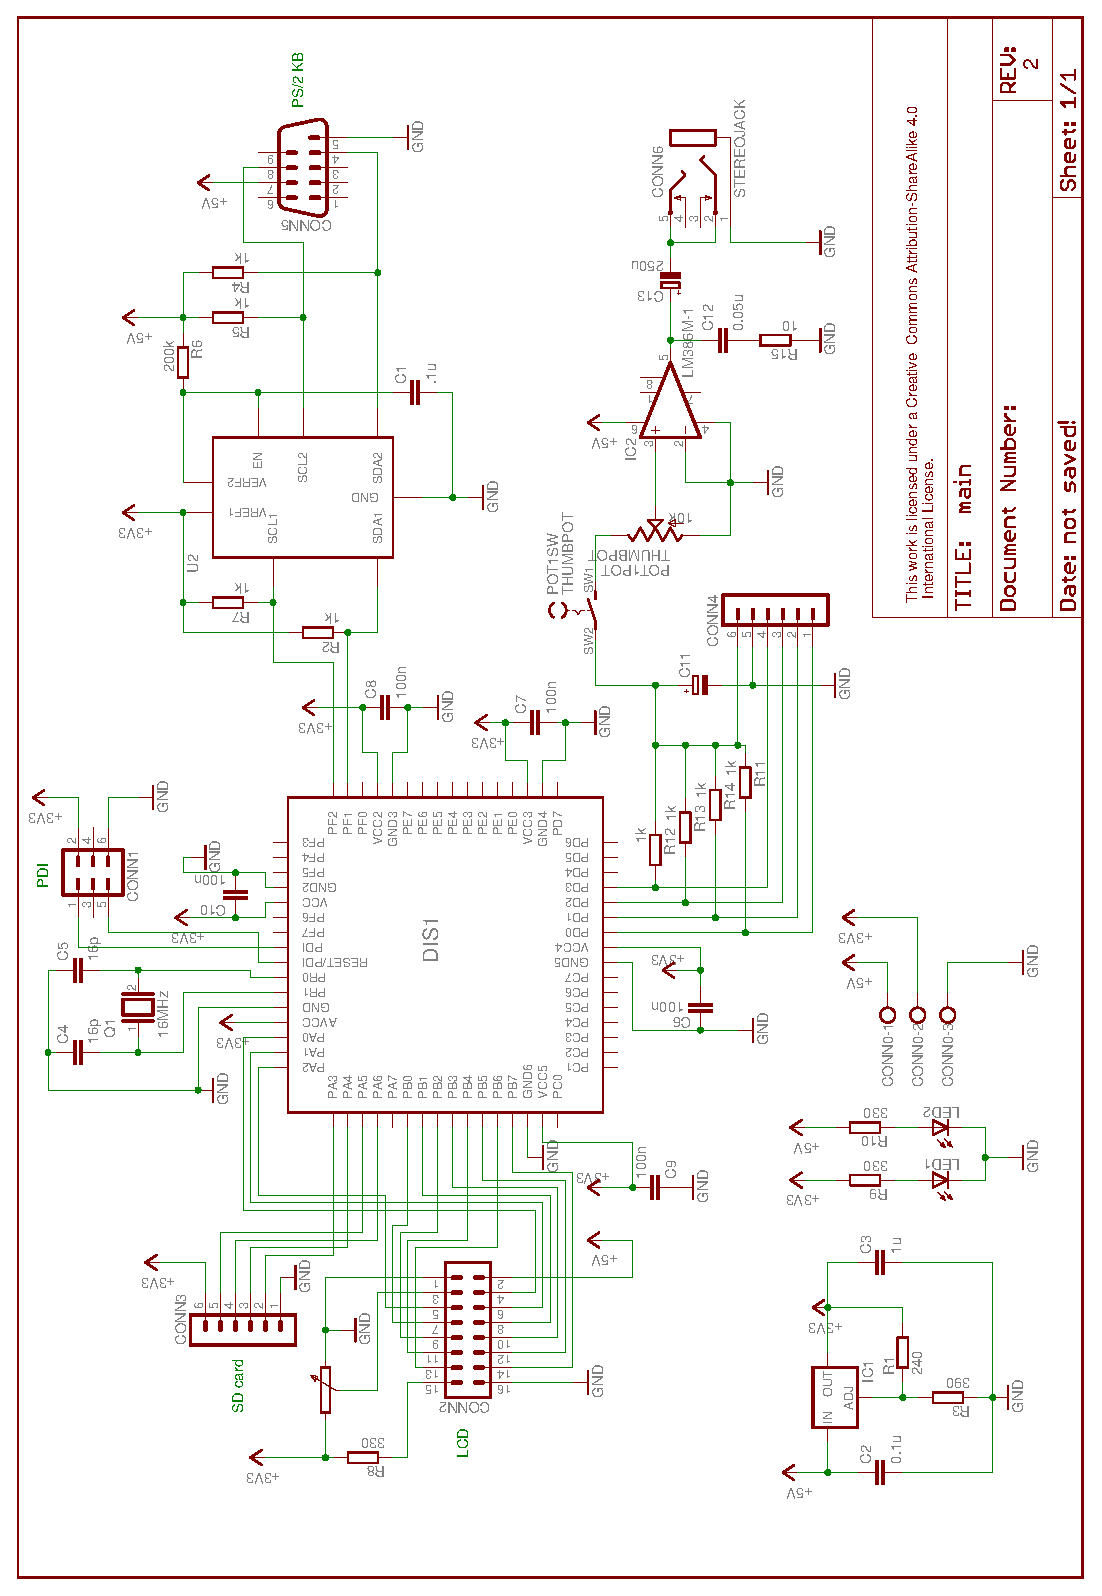
\includegraphics[width=0.9\linewidth]{img/fig_full_schematic}
        \caption{Full Schematic}
    \end{figure}
    \clearpage
      \begin{figure}[H]
        \centering
          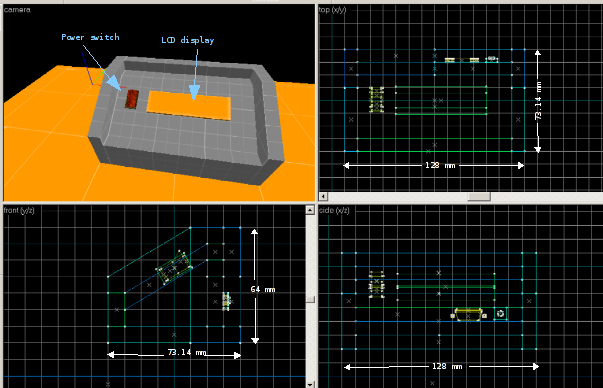
\includegraphics[width=\linewidth]{img/fig_mechanical0}
          \caption{Mechanical schematic of enclosure}
          \label{fig:3d1}
      \end{figure}
      \begin{figure}[H]
        \centering
          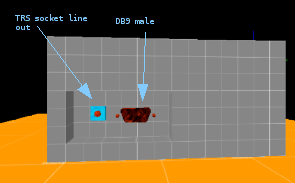
\includegraphics[width=\linewidth]{img/fig_mechanical1}
          \caption{Rear 3D view of enclosure}
          \label{fig:3d2}
      \end{figure}
\section{Large Software Diagrams}
    \begin{figure}[H]
      \centering
        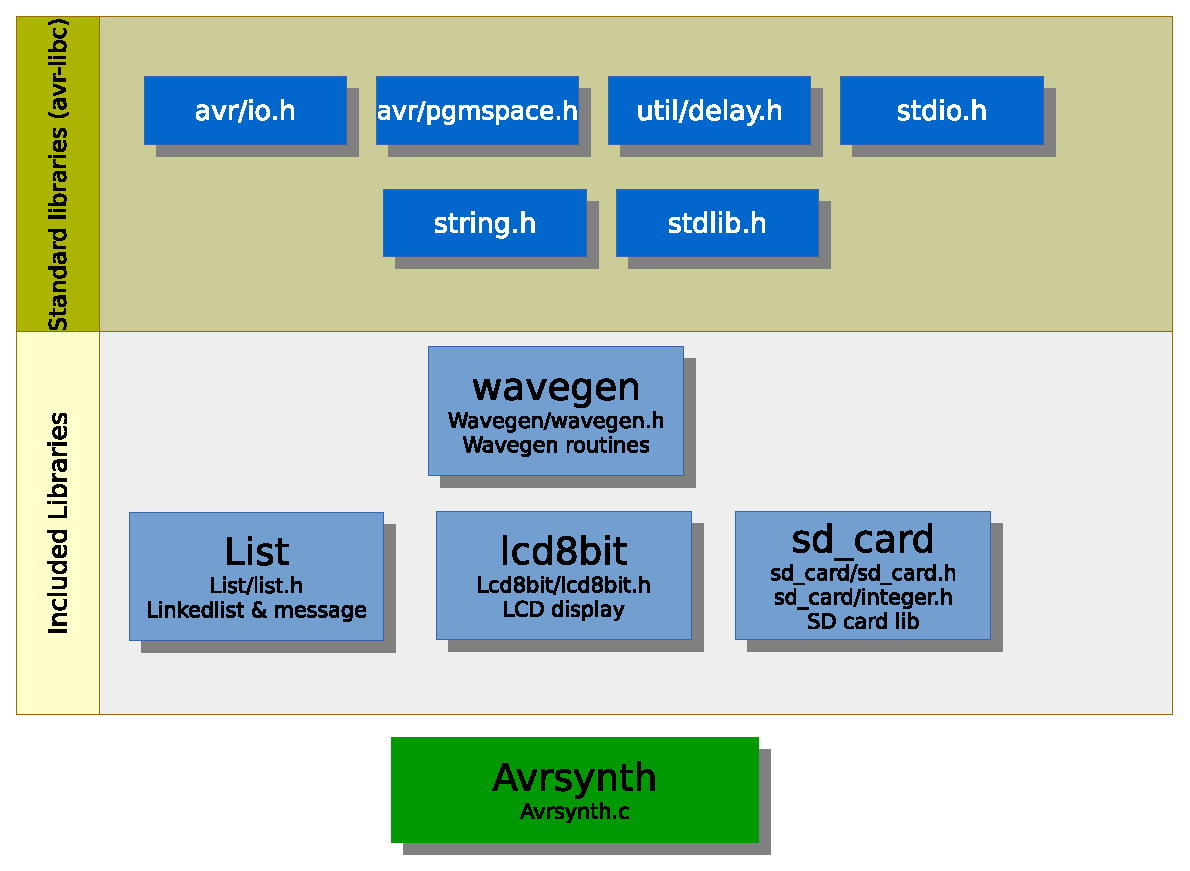
\includegraphics[width=\linewidth]{img/fig_soft_diag}
        \caption{High Level Software Topology}
    \end{figure}
    \begin{figure}[H]
      \centering
        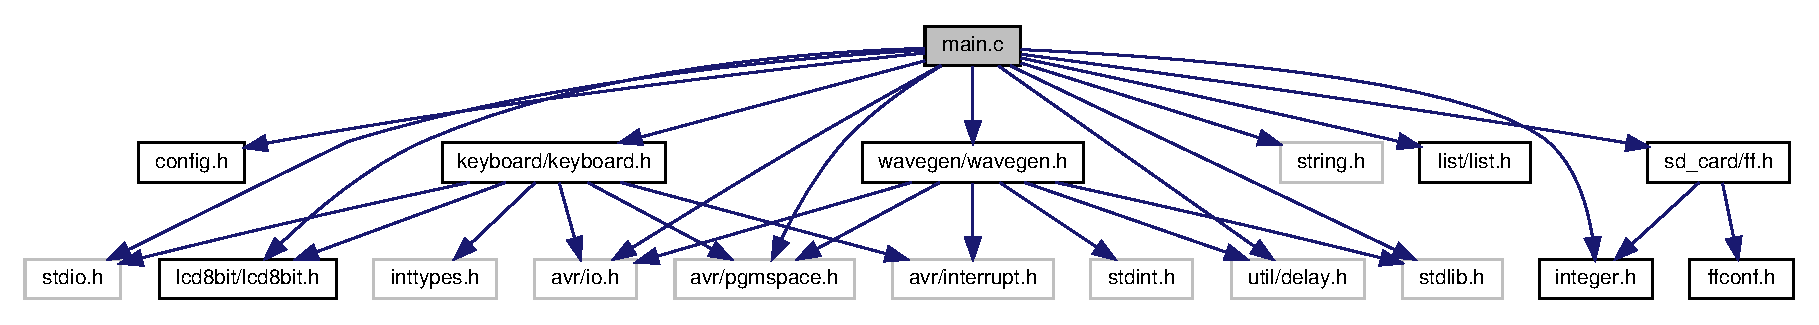
\includegraphics[width=\linewidth]{img/main_8c_incl.eps}
        \caption{Include dependency graph for main.c}
    \end{figure}
    \begin{figure}[H]
      \centering
        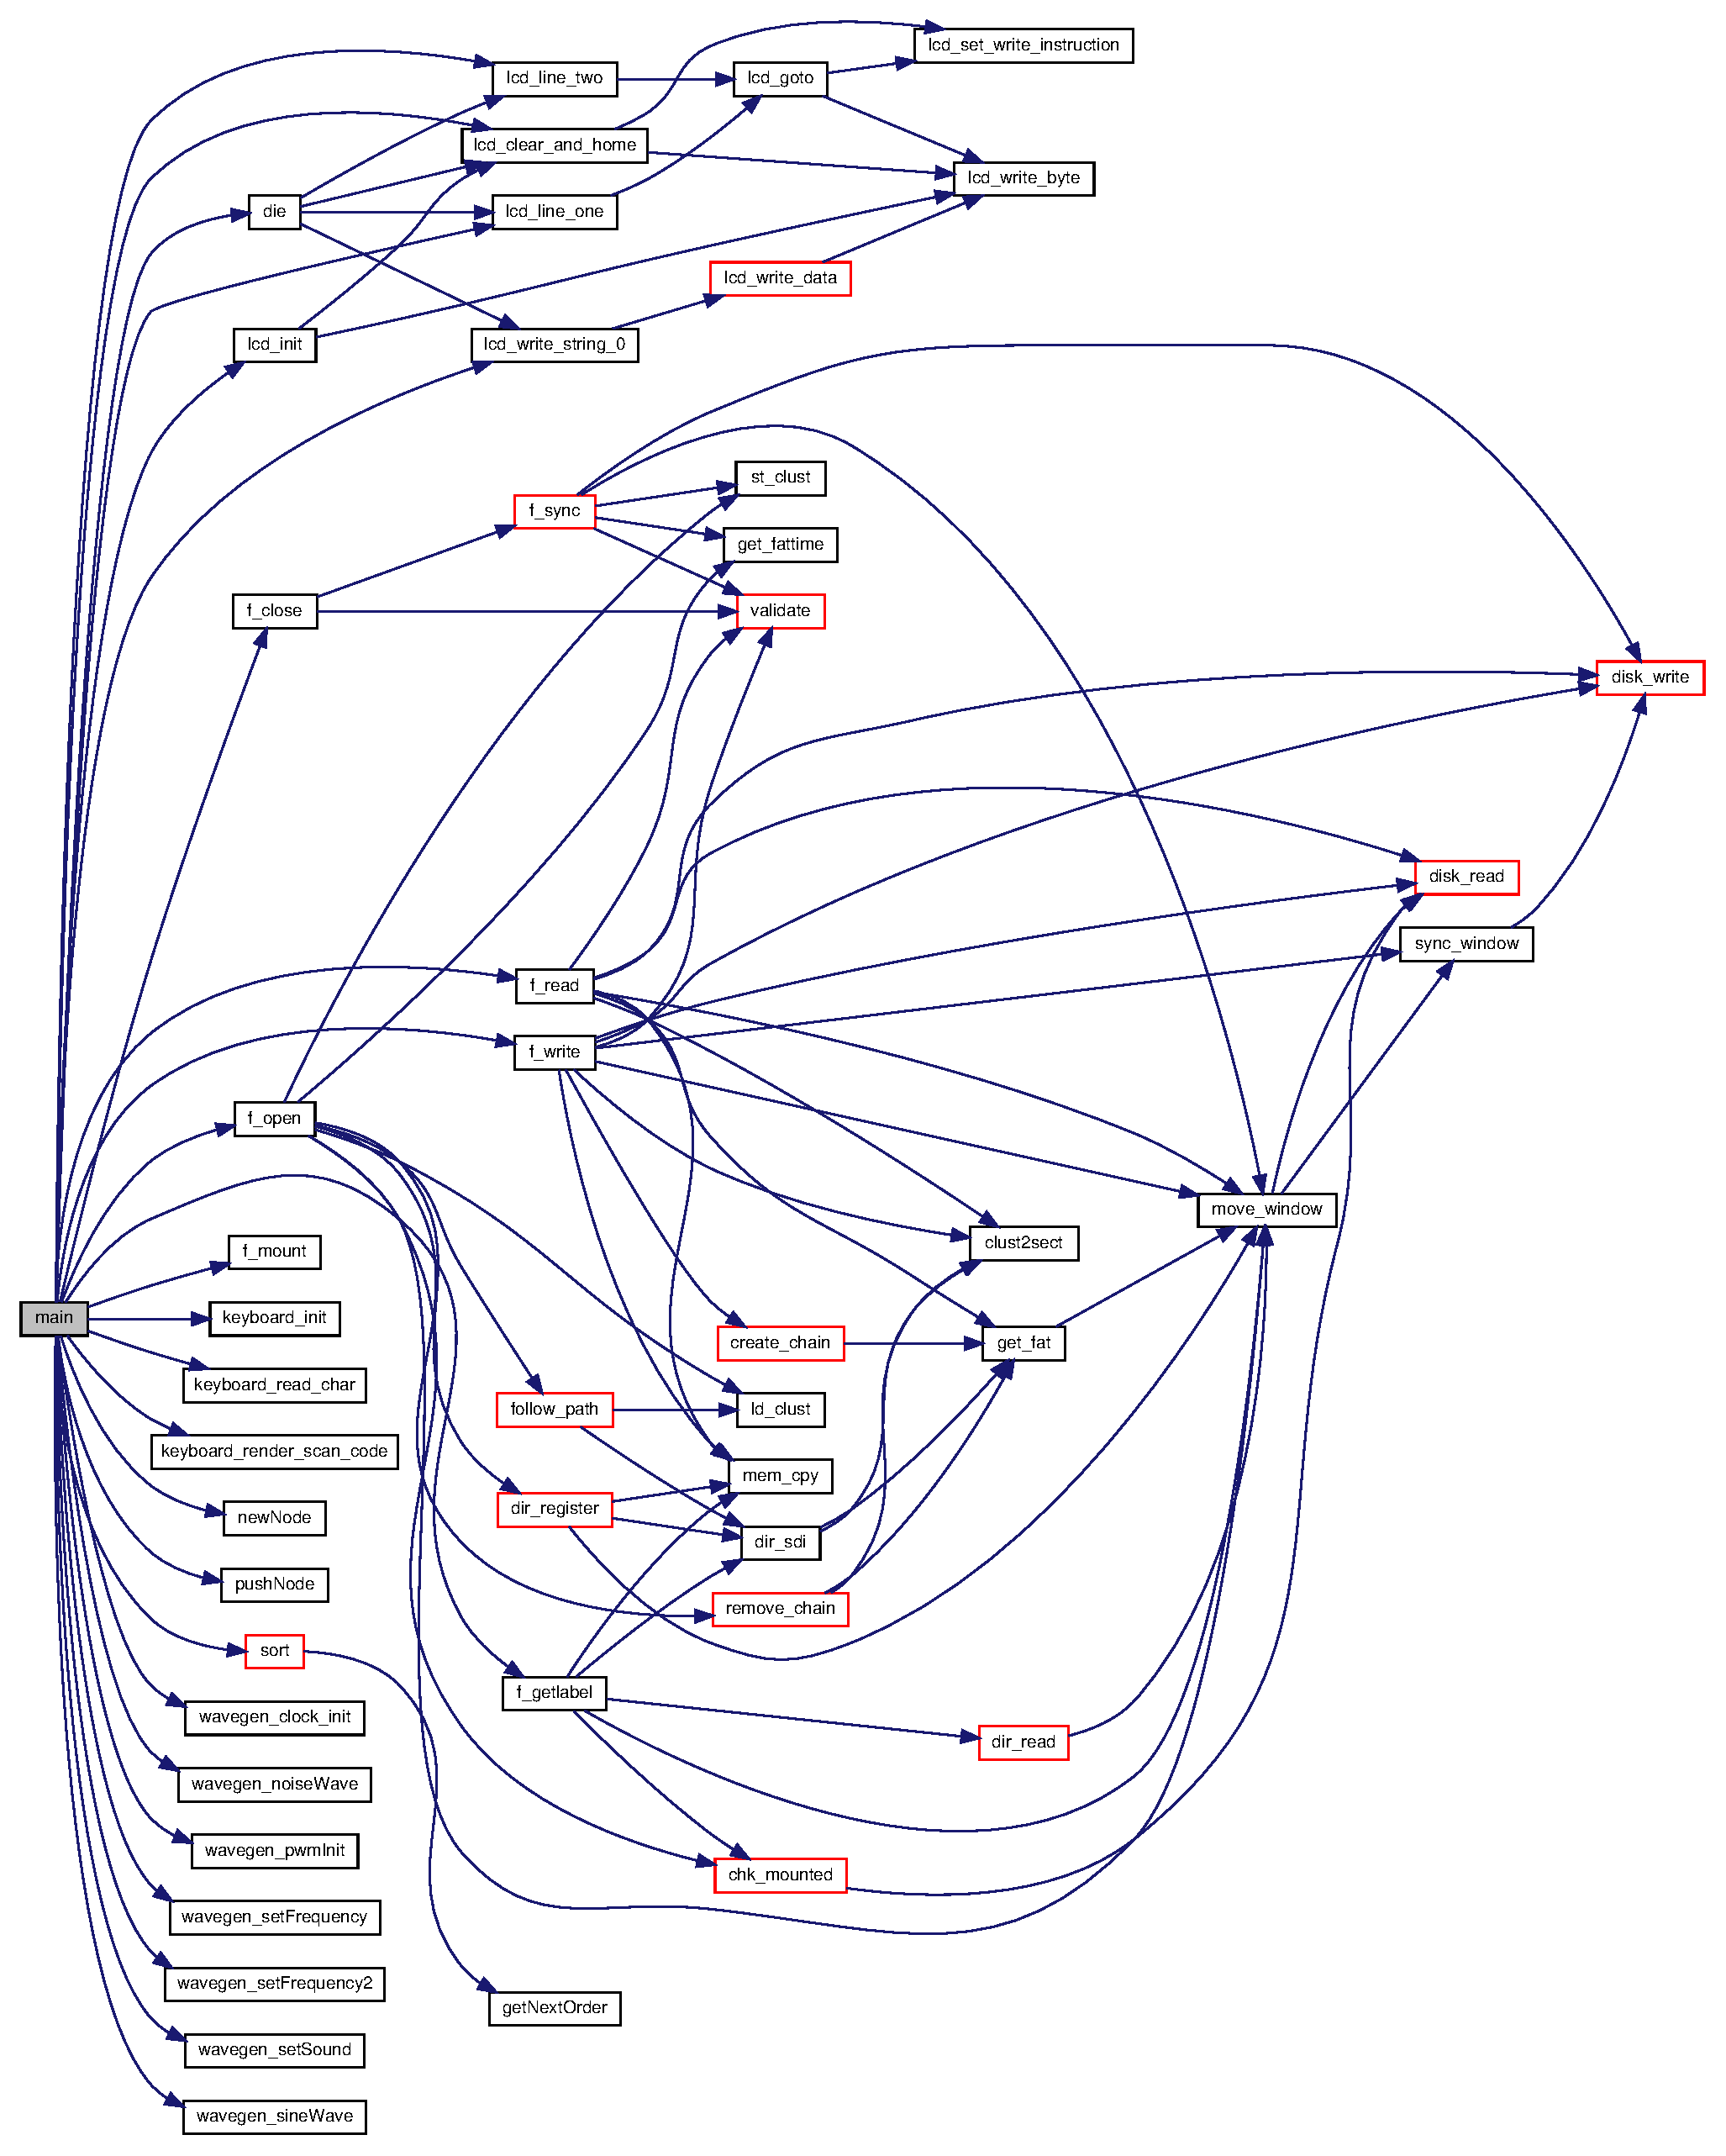
\includegraphics[width=\linewidth]{img/main_8c_ae66f6b31b5ad750f1fe042a706a4e3d4_cgraph.eps}
        \caption{Callgraph for int main()}
    \end{figure}

    \clearpage
\section{Large Software Listings}
\begin{lstlisting}[frame=single,caption=Avrsynth project makefile,style=makefile]
DEVICE = atxmega256d3
AVRDUDE_DEVICE =x256d3

PROG = -c avrispmkII -P usb

CFLAGS=-g -Wall -mcall-prologues -mmcu=$(DEVICE) -Os
CC=avr-gcc
OBJ2HEX=avr-objcopy
LDFLAGS=-Wl,-gc-sections -Wl,-relax

AVRDUDE=avrdude
TARGET=main
OBJECT_FILES=main.o
SRC_FILES=$(OBJECT_FILES:%.o=%.c)

  all: $(TARGET).hex

  clean:
          rm -f *.o *.hex *.obj *.hex

          %.hex: %.obj
                  $(OBJ2HEX) -R .eeprom -O ihex $< $@

                  %.obj: $(OBJECT_FILES)
          $(CC) $(CFLAGS) $(OBJECT_FILES) $(LDFLAGS) -o $@

          program: $(TARGET).hex
                  $(AVRDUDE) -p $(AVRDUDE_DEVICE) $(PROG) -U flash:w:$(TARGET).hex
\end{lstlisting}
\begin{lstlisting}[frame=single,caption=Snippet from avrsynth.c performing frequency generation from list structure,style=customc]
sineWave();
clock_init();
pwmInit();
PORTD.DIRSET=0xFF;
struct order* gett = (getOrderNode(head,1)->data);
setFrequency2(getOrderFrequency(gett));

gett = (getOrderNode(head,2)->data);
setFrequency(getOrderFrequency(gett));
unsigned long count=0;
unsigned int count_ms=0;

//10 sec of music
while(1)
{
  count++;
  if((count == 320000))
  {
    count=0;
    count_ms++;
    //freq step
  }
  //noiseWave();
  //wait here
}
\end{lstlisting}

  \clearpage
\section{Calibration Instructions}
N/A
  \clearpage
\section{Datasheets}
N/A
\clearpage
%\textit{Note: When printed out for final report, datasheets shall appear as pages}
%  \begin{enumerate}
%    \item{atxmega256D3 - \scriptsize\url{http://www.atmel.com/Images/Atmel-8134-8-16-bit-Atmel-XMEGA-D3-Microcontroller\_Datasheet.pdf}}
%    \item{LCD QC1602A display - \scriptsize\url{http://www.mpja.com/download/QC1602a.pdf}}
%    \item{SD card slot \scriptsize\url{http://dlnmh9ip6v2uc.cloudfront.net/datasheets/Components/General/SDMMCCardSock.pdf}
%      \scriptsize\url{http://www.geeetech.com/wiki/index.php/Arduino\_SD\_card\_Module}}
%    \item{FAT\_FS - \scriptsize\url{http://www.pocketmagic.net/2013/08/avr-sdcard-fat-support-with-fatfs/}}
%    \item{PCA9306DCTR I2C bus level shifter for PS/2 \scriptsize\url{http://www.ti.com/product/pca9306}}
%    \item{LM317 adjustable voltage regulator \scriptsize\url{http://www.ti.com/product/lm317}}
%  \end{enumerate}
%  \clearpage

\section{Subsystem Unit Tests}
      \begin{table}[H]
      \small
      \caption{LCD unit test}
      \label{tab:lcd_unittest}
      \begin{tabularx}{\textwidth}{ |p{2.1cm}|L|L|p{0.7cm}|p{0.6cm}|X| }
        \hline
        \multicolumn{2}{|l|}{\textbf{Test Writer}} & \multicolumn{4}{c|}{Matt Bagnara} \\
        \hline
        \multicolumn{2}{|l|}{\textbf{Test Case Name}} & {LCD unit test} & \multicolumn{2}{c|}{\textbf{Type}} & subsystem \\
        \hline
        \textbf{Description} & \multicolumn{2}{|>{\centering\setlength\hsize{2\hsize} }X|}{Verify correct communication of ASCII text to display screen} & \multicolumn{2}{c|}{\textbf{Date}} & 09/25/13 \\
        \hline
        \textbf{Setup} & \multicolumn{2}{|>{\centering\setlength\hsize{2\hsize} }X|}{Connect LCD tester using pinout displayed in Appendix J} & \multicolumn{2}{c|}{\textbf{Time}} & 22:12\\
        \hline
        \multicolumn{6}{|l|}{\textbf{Test}} \\
        \hline
        \textbf{Name} & \textbf{Action} & \textbf{Expected output} & \textbf{Pass} & \multicolumn{2}{X|}{\textbf{Comments}} \\
        \hline
        Poweron test & Apply power to microcontroller & Display lights up? & \checkmark & \multicolumn{2}{X|}{} \\
        \hline
        ASCII test & No action needed & Will display an ASCII message on LCD & \checkmark & \multicolumn{2}{X|}{} \\
        \hline
        Control character test & No action needed & Will display custom characters on the LCD & \checkmark & \multicolumn{2}{X|}{} \\
        \hline
        Contrast adjust & Adjust rheostat on tester board & Contrast should adjust on screen & \checkmark & \multicolumn{2}{X|}{} \\
        \hline
      \end{tabularx}
      \end{table}

      \begin{table}[H]
      \small
      \caption{PS/2 interface unit test}
      \label{tab:ps2_unittest}
      \begin{tabularx}{\linewidth}{ |p{2.1cm}|L|L|p{0.7cm}|p{0.6cm}|L| }
        \hline
        \multicolumn{2}{|l|}{\textbf{Test Writer}} & \multicolumn{4}{c|}{Matt Bagnara} \\
        \hline
        \multicolumn{2}{|l|}{\textbf{Test Case Name}} & {PS/2 Keyboard interface} & \multicolumn{2}{c|}{\textbf{Type}} & subsystem \\
        \hline
        \textbf{Description} & \multicolumn{2}{|>{\centering\setlength\hsize{2\hsize} }X|}{Test user input via PS/2 keyboard input} & \multicolumn{2}{c|}{\textbf{Date}} & 09/20/13 \\
        \hline
        \textbf{Setup} & \multicolumn{2}{|>{\centering\setlength\hsize{2\hsize} }X|}{Connect processor power and setup as in Appendix J} & \multicolumn{2}{c|}{\textbf{Time}} & 14:22\\
        \hline
        \multicolumn{6}{|l|}{\textbf{Test}} \\
        \hline
        \textbf{Name} & \textbf{Action} & \textbf{Expected output} & \textbf{Pass} & \multicolumn{2}{X|}{\textbf{Comments}} \\
        \hline
        PS/2 poweron test & Power microcontroller & Keyboard LEDs should light up initially and turn off & \checkmark & \multicolumn{2}{X|}{} \\
        \hline
        Key press event & Press any alphanumeric key on keyboard & LEDs should light indicated scancode. See PS/2 scancode list.& \checkmark & \multicolumn{2}{X|}{} \\
        \hline
        Key release event & Release any alphanumeric key on the keyboard & LEDs should light indicated scancode. See PS/2 scancode list.& \checkmark & \multicolumn{2}{X|}{} \\
        \hline
        Contrast adjust & Adjust rheostat on tester board & Contrast should adjust on screen & \checkmark & \multicolumn{2}{X|}{} \\
        \hline
      \end{tabularx}
      \end{table}

      \begin{table}[H]
      \small
      \caption{SD storage unit test}
      \label{tab:sd_unittest}
      \begin{tabularx}{\linewidth}{ |p{2.1cm}|L|L|p{0.7cm}|p{0.6cm}|X| }
        \hline
        \multicolumn{2}{|l|}{\textbf{Test Writer}} & \multicolumn{4}{c|}{Matt Bagnara} \\
        \hline
        \multicolumn{2}{|l|}{\textbf{Test Case Name}} & {SD storage interface} & \multicolumn{2}{c|}{\textbf{Type}} & subsystem \\
        \hline
        \textbf{Description} & \multicolumn{2}{|>{\centering\setlength\hsize{2\hsize} }X|}{Test reading of data from SD interface} & \multicolumn{2}{c|}{\textbf{Date}} & 10/09/13 \\
        \hline
        \textbf{Setup} & \multicolumn{2}{|>{\centering\setlength\hsize{2\hsize} }X|}{Connect processor power and setup as in Appendix J} & \multicolumn{2}{c|}{\textbf{Time}} & 17:32\\
        \hline
        \multicolumn{6}{|l|}{\textbf{Test}} \\
        \hline
        \textbf{Name} & \textbf{Action} & \textbf{Expected output} & \textbf{Pass} & \multicolumn{2}{X|}{\textbf{Comments}} \\
        \hline
        SD library initialize & Power microcontroller & LED on PORTC should light & \checkmark & \multicolumn{2}{X|}{} \\
        \hline
        SD library read block & Power microcontroller & Test should read ASCII data off SD card and turn back LED on PORTC & \checkmark & \multicolumn{2}{X|}{} \\
        \hline
      \end{tabularx}
      \end{table}

      \begin{table}[H]
      \small
      \caption{Synthesis unit test}
      \label{tab:synthesis_unittest}
      \begin{tabularx}{\linewidth}{ |p{2.1cm}|L|L|p{0.7cm}|p{0.6cm}|X| }
        \hline
        \multicolumn{2}{|l|}{\textbf{Test Writer}} & \multicolumn{4}{c|}{Matt Bagnara} \\
        \hline
        \multicolumn{2}{|l|}{\textbf{Test Case Name}} & {Synthesis unit test} & \multicolumn{2}{c|}{\textbf{Type}} & subsystem \\
        \hline
        \textbf{Description} & \multicolumn{2}{|>{\centering\setlength\hsize{2\hsize} }X|}{Includes conversion of digital wavetable data into a synthesized waveform} & \multicolumn{2}{c|}{\textbf{Date}} & 10/09/13 \\
        \hline
        \textbf{Setup} & \multicolumn{2}{|>{\centering\setlength\hsize{2\hsize} }X|}{Connect processor power and setup as in Appendix J} & \multicolumn{2}{c|}{\textbf{Time}} & 17:32\\
        \hline
        \multicolumn{6}{|l|}{\textbf{Test}} \\
        \hline
        \textbf{Name} & \textbf{Action} & \textbf{Expected output} & \textbf{Pass} & \multicolumn{2}{X|}{\textbf{Comments}} \\
        \hline
        Frequency test & Run single tone example & 440Hz & X & \multicolumn{2}{X|}{Still needs further calibration} \\
        \hline
        Frequncy sweep & Select Freq sweep in debug menu & sweep from 40 to 10000Hz in 10 seconds & X & \multicolumn{2}{X|}{current implementation} \\
        \hline
        Noise generation & Run noise-gen routine & continous noise output & \checkmark & \multicolumn{2}{X|}{} \\
        \hline
        Two tones & Run two-tone routine & 440Hz and 460Hz & \checkmark & \multicolumn{2}{X|}{} \\
        \hline
        Three tones & Run tri-tone routine & 440Hz 460Hz 520Hz & \checkmark & \multicolumn{2}{X|}{} \\
        \hline
        Frequency test & Run single tone example & 440Hz & X & \multicolumn{2}{X|}{Still needs further calibration} \\
        \hline
        Squrare generation & Run square-gen routine & continuous squarewave at 440Hz 50\% duty  & \checkmark & \multicolumn{2}{X|}{} \\
        \hline
        Triangle generation & Run triangle-gen routine & continous triangle wave at 440Hz & X & \multicolumn{2}{X|}{In progress} \\
        \hline
      \end{tabularx}
      \end{table}
      
      \begin{table}[H]
      \small
      \caption{Processor unit test}
      \label{tab:processor_unittest}
      \begin{tabularx}{\linewidth}{ |p{2.1cm}|L|L|p{0.7cm}|p{0.6cm}|X| }
        \hline
        \multicolumn{2}{|l|}{\textbf{Test Writer}} & \multicolumn{4}{c|}{Matt Bagnara} \\
        \hline
        \multicolumn{2}{|l|}{\textbf{Test Case Name}} & {Processor platform test} & \multicolumn{2}{c|}{\textbf{Type}} & subsystem \\
        \hline
        \textbf{Description} & \multicolumn{2}{|>{\centering\setlength\hsize{2\hsize} }X|}{Includes demonstration of processor functionality as a hardware platform} & \multicolumn{2}{c|}{\textbf{Date}} & 11/10/13 \\
        \hline
        \textbf{Setup} & \multicolumn{2}{|>{\centering\setlength\hsize{2\hsize} }X|}{Connect processor power and setup as in Appendix J} & \multicolumn{2}{c|}{\textbf{Time}} & 12:27\\
        \hline
        \multicolumn{6}{|l|}{\textbf{Test}} \\
        \hline
        \textbf{Name} & \textbf{Action} & \textbf{Expected output} & \textbf{Pass} & \multicolumn{2}{X|}{\textbf{Comments}} \\
        \hline
        Poweron test & Power microcontroller & 1.7V to 3.6V on VCC and AVCC pin & \checkmark & \multicolumn{2}{X|}{} \\
        \hline
        PDI interface advertisement & See \scriptsize\nameref{processortest} & Should respond with device signature \texttt{0x1e9844} & \checkmark & \multicolumn{2}{X|}{} \\
        \hline
      \end{tabularx}
      \end{table}
\clearpage
\section{Testing Documentation}
      \label{sec:testing-documentation}
  \begin{enumerate}
    \item{\textbf{LCD Tester}}\hfill \\
    The data bits are connected to PORTA. The control bits are connected to PORTD[7..5]. A common ground and +5V must be established between the microcontroller and the testing board.\par

      The microcontroller will be loaded with the 'lcd8bit' hex file and will complete the tests automatically upon running. The microcontroller will display a short message on the first line of the display. Following, custom glyph characters will be displayed on the second line of the display. The core functionality of the display such as clearing and modifying will be done using these tests.
  \begin{figure}[H]
    \centering
      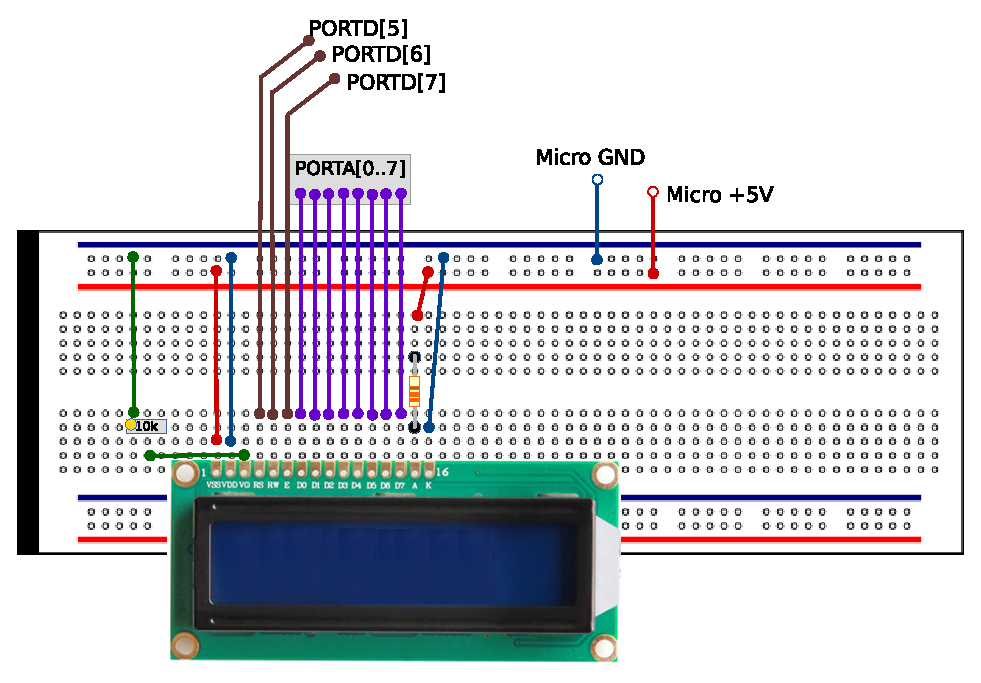
\includegraphics[width=\linewidth]{img/testdoc_lcdtester}
      \caption{LCD tester layout}
  \end{figure}

    \item{\textbf{PS/2 Keyboard Tester}}\hfill \\
    The PS/2 keyboard will be connected to the 6-pin mini DIN connector which is coupled to the microcontroller board. The mini DIN requires an adaptor to DB-9 to connect easily for testing. For the usage of the test, a DB-9 to mini-DIN adaptor dongle will be used. The dongle connector is wired as follows:
  \begin{figure}[H]
    \centering
      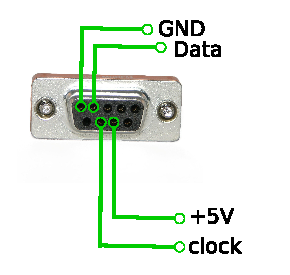
\includegraphics[]{img/testdoc_dongle}
      \caption{PS/2 Dongle pinout}
  \end{figure}

    The opposite side of the connector will be jumpered to the microcontroller board on PORTB; with clock being B.2 and data being B.1. A common ground and +5V must be established between the microcontroller and the testing board.

    The PS/2 tester will display the regular scancode for the last key being pressed or released on the LEDs using PORTC. The press and release scancodes are displayed here.
    \item{\textbf{SD Card Tester}}\hfill \\
    The SD card breakout board will be connected using jumper connections to the microcontroller board. Because the SD breakout board includes a level converter, there is no voltage issue using +5V. The wiring is shown. PORTB is used for to connect to the breakout board. The SD is inserted into the slow when powered down. Only regular SD cards may be used with size up to 1GB.
  \begin{figure}[H]
    \centering
      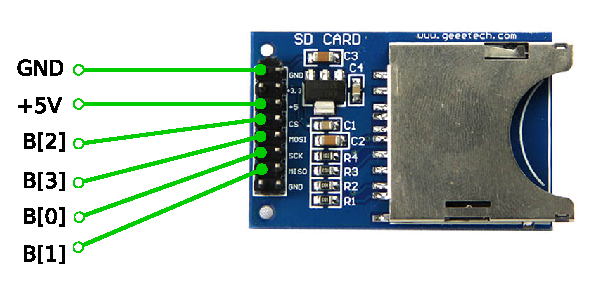
\includegraphics[]{img/testdoc_sd}
      \caption{SD board pinout}
  \end{figure}

    The microcontroller is loaded with the 'sd\_test.hex' hex file and powered with the SD card in place.
    \item{\textbf{Processor}}\hfill \\
    The processor testing environment is established through a rudimentary PDI programming interface. The essential build environment requires this interface and a powered processor. With a fundamental environment created, it is possible to verify communication via the PDI programmer. This test will make use of the AVRISP mkII programmer.

      The first test requires a verification of the processor device. This consists of a request by the development workstation and a simple reply advertisement by the processor. This can be simply executed by issuing \texttt{avrdude -p x256d3 -c avriskmkII -P usb} in the terminal of the workstation. A valid response from the processor would be a device signature of \texttt{0x1e9844} when using the ATXMEGA256D3.
      \label{processortest}

    \item{\textbf{Integration Platform}}\hfill \\
      The integration platform was designed for use throughout the subsystem integration phase of the project. Each individual hardware subsystem can be exclusively attached and detached from the platform. This allows comparative testing to be done using any integration regression.

      Standard connections are as follows:

    \begin{table}[H]
    \caption{Development board connections}
    \vskip 0.3cm
    \small
    \center
    \begin{tabularx}{0.8\textwidth}{  l X }
      \textbf{Connection} & \textbf{Description}\\
      \hline
      CONN1 & PDI interface\\
      CONN2 & LCD\\
      CONN3 & SD interface\\
      CONN4 & Wave generation PWM\\
      CONN5 & PS/2 I2C interface\\
      CONN6 & Production power terminal\\
      CONN7 & Power terminal (+3.3V,GND,+5V)\\
      DIS1 & Xmega-compatible 64-pin processor assembly card\\
    \end{tabularx}
    \end{table}
  \begin{figure}[H]
    \centering
      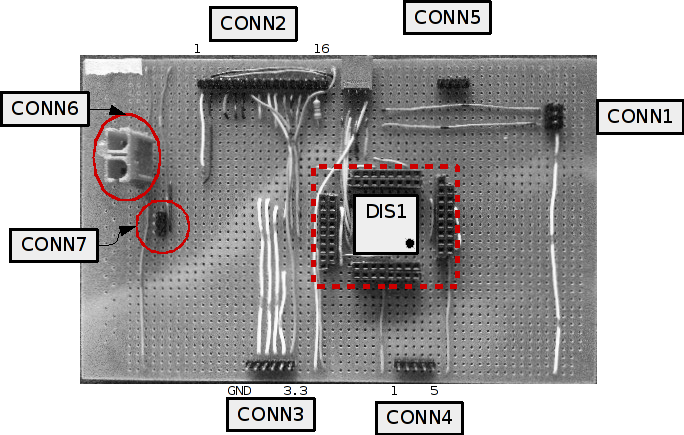
\includegraphics[width=\linewidth]{img/testdoc_board}
      \caption{Development board}
  \end{figure}
\end{enumerate}
\clearpage
\section{Licenses}
\begin{enumerate}

  \item{\textbf{Hardware design:}}\hfill \\
    The hardware for this project is licensed under the Creative Commons Attribution-ShareAlike 4.0 International License.

    \url{http://creativecommons.org/licenses/by-sa/4.0/}

    \includegraphics[width=1in]{img/by-sa.eps}

  \item{\textbf{Software design:}}\hfill \\
    The software for this project is licensed under the GNU General Public License Version 3 (GPLv3):

    This program is free software: you can redistribute it and/or modify
    it under the terms of the GNU General Public License as published by
    the Free Software Foundation, either version 3 of the License, or
    (at your option) any later version.
    This program is distributed in the hope that it will be useful,
    but WITHOUT ANY WARRANTY; without even the implied warranty of
    MERCHANTABILITY or FITNESS FOR A PARTICULAR PURPOSE.  See the
    GNU General Public License for more details.
    You should have received a copy of the GNU General Public License
    along with this program.  If not, see \url{http://www.gnu.org/licenses/}.
      
    
\includegraphics[width=1in]{img/gpl_logo.png}


    \item{\textbf{Creative Content:}}\hfill \\
    The creative content for this project includes the title, artwork or display of the project, graphics, illustrations, pictoral representations, etc. All are licensed under the Creative Commons Attribution-ShareAlike 4.0 International License.

    \url{http://creativecommons.org/licenses/by-sa/4.0/}

    \includegraphics[width=1in]{img/by-sa.eps}\\

    \item{\textbf{Documentation:}}\hfill \\
    The documentation for this project includes development documentation, testing documentation, written or digital, and this report. All are licensed under the Creative Commons Attribution 4.0 International License.

    \url{http://creativecommons.org/licenses/by/4.0/}

    \includegraphics[width=1in]{img/by.eps}

\end{enumerate}

% ------------------------------------------------------------------------------
% End document
% ------------------------------------------------------------------------------
\end{document}

